\subsection{Indecomposable Modules and Primordial Modules}

Let A be a ring. Recall the following definition (VII, §4, No.~8, p.~23, Definition 3).

DEFINITION 2. --- An A-module M is called indecomposable if it is not the direct sum of a family of submodules distinct from 0 and M.

By the corollary of Proposition 12 of II, §1, No.~8, p.~209, the following properties are equivalent:

\begin{enumerate}
\def\labelenumi{\alph{enumi})}
\item
  The A-module M is indecomposable.
\item
  The A-module M is nonzero, and every direct factor submodule of M is equal to 0 or M.
\item
  The A-module M is nonzero, and the ring \(\operatorname{End}_{\mathrm{A}}(\mathrm{M})\) contains no idempotent distinct from 0 and \(1_{M}\) .
\end{enumerate}

In particular, since the endomorphism ring of the A-module \(A_{s}\) is isomorphic to the opposite ring of A, we see that the A-module \(A_{s}\) is indecomposable if and only if the ring A is nonzero and its only idempotents are 0 and 1.

Example. --- Suppose that the ring A is a principal ideal domain. The indecomposable finitely generated A-modules are the A-modules isomorphic to either A or \(A/p^{n}A\) , where p is an irreducible element of A and n an integer \textgreater0 (VII, §4, No.~8, p.~24, Proposition 8).

PROPOSITION 3. --- A Noetherian or Artinian A-module M is the direct sum of a finite family of indecomposable submodules.

Let us first prove that every nonzero submodule P of M has an indecomposable direct factor. If this were not the case, then every direct factor submodule of P would be decomposable; proceeding by induction, we could then construct, for every \(n \in N\) , nonzero submodules \(N_{n}^{\prime}\) and \(N_{n}^{\prime\prime}\) of P such that \(P = N_{0}^{\prime} \oplus N_{0}^{\prime\prime}\) and \(N_{n-1}^{\prime} = N_{n}^{\prime} \oplus N_{n}^{\prime\prime}\) for \(n \geqslant 1\) . But then, the sequence of submodules \(N_{0}^{\prime\prime} + \cdots + N_{n}^{\prime\prime}\) would be strictly increasing, and that of the submodules \(N_{n}^{\prime}\) would be strictly decreasing. The module M would be neither Noetherian nor Artinian, contrary to the assumption.

Now, suppose that M is not the direct sum of a finite family of indecomposable submodules. By induction, we construct indecomposable submodules \(P_{n}^{\prime\prime}\) of M and nonzero submodules \(P_{n}^{\prime}\) of M for every \(n \in N\) such that \(M = P_{0}^{\prime} \oplus P_{0}^{\prime\prime}\) and \(P_{n-1}^{\prime} = P_{n}^{\prime} \oplus P_{n}^{\prime\prime}\) for \(n \geqslant 1\) . Indeed, M is nonzero, and the first part of the proof, applied to P = M, provides \(P_{0}^{\prime}\) and \(P_{0}^{\prime\prime}\) . Since the modules \(P_{k}^{\prime}\) and \(P_{k}^{\prime\prime}\) are defined for k \textless{} n, by the first part of the proof, there exist submodules \(P_{n}^{\prime}\) and \(P_{n}^{\prime\prime}\) such that \(P_{n-1}^{\prime} = P_{n}^{\prime} \oplus P_{n}^{\prime\prime}\) with \(P_{n}^{\prime\prime}\) indecomposable. The relation \(M = P_{n}^{\prime} \oplus P_{0}^{\prime\prime} \oplus \cdots \oplus P_{n}^{\prime\prime}\) then implies that \(P_{n}^{\prime} \neq 0\) because M is not the direct sum of a finite family of indecomposable modules.

The sequence of submodules \(P_{0}^{\prime\prime} \oplus \cdots \oplus P_{n}^{\prime\prime}\) is strictly increasing, and the sequence of submodules \(P_{n}^{\prime}\) is strictly decreasing. This contradicts the assumption that M is Noetherian or Artinian.

The question of the uniqueness of the decomposition of a module as a direct sum of indecomposable submodules will be studied in the next subsection.

DEFINITION 3. --- A module is called primordial \(^{(1)}\) if its endomorphism ring is local.

By definition, a local ring is not reduced to 0; consequently, a primordial module is nonzero. Moreover, the A-module \(A_{s}\) is primordial if and only if the ring A is local.

PROPOSITION 4. --- a) A primordial module is indecomposable.

\begin{enumerate}
\def\labelenumi{\alph{enumi})}
\setcounter{enumi}{1}
\tightlist
\item
  An indecomposable module of finite length is primordial.
\end{enumerate}

Let M be an A-module. Suppose that M is primordial; let e be an idempotent in the local ring \(\operatorname{End}_{\mathrm{A}}(\mathrm{M})\) . Since \(e^{2}=e\) , either e is invertible and we have e=1, or 1-e is invertible and we have e=0. This proves that M is indecomposable (VIII, p.~30).

Now, suppose that M is indecomposable and of finite length. By Proposition 2, c) of VIII, p.~27, every endomorphism of M is invertible or nilpotent; the ring \(\operatorname{End}_{\mathrm{A}}(\mathrm{M})\) is therefore local by Example 2 of VIII, p.~26.

The Z-module Z is indecomposable, Noetherian, but not Artinian. Its endomorphism ring is isomorphic to Z, hence is not local. Consequently, Z is not a primordial Z-module.

*Let \(p\) be a prime number. The endomorphism ring of the \(\mathbf{Z}\) -module \(\mathbf{Q}_p / \mathbf{Z}_p\) is isomorphic to the local ring \(\mathbf{Z}_p\) (cf.~VII, §4, p.~65, Exercise 13); it is therefore a primordial \(\mathbf{Z}\) -module.

An injective module is indecomposable if and only if it is primordial (X, §1, n° 9, p.~21, proposition 14).*

\subsection{Semiprimordial Modules}

DEFINITION 4. --- A module is called semiprimordial if it is the direct sum of a family of primordial submodules.

*Examples. --- 1) Every simple module is primordial (VIII, p.~45); every semisimple module is therefore semiprimordial (VIII, p.~55, Definition 1).

\begin{enumerate}
\def\labelenumi{\arabic{enumi})}
\setcounter{enumi}{1}
\tightlist
\item
  If A is a left Noetherian ring, then every injective A-module is semiprimordial (X, §1, n° 9, p.~21, proposition 14 and X, §1, n° 10, p.~22, théorème 3, b)).*
\end{enumerate}

THEOREM 1 (Azumaya). --- Let A be a ring, L a primordial A-module, and M a semiprimordial A-module. There exists a unique cardinal, denoted by {[}M : L{]}, with the following property:

For every decomposition \(M = \bigoplus_{i \in I} M_i\) of M as a direct sum of primordial modules, the set of indices \(i \in I\) such that \(M_i\) is isomorphic to L has cardinal {[}M : L{]}.

The proof is based on the following four lemmas.

Lemma 1. --- Let M be an A-module, M' a primordial submodule of M, and M'\,' a submodule of M supplementary to M'. Let u be an endomorphism of M. Then u or \(1_{M} - u\) induces an isomorphism from M' to a submodule of M supplementary to M'\,'.

Let \(p\) be the projection from M onto \(M'\) with kernel \(M''\) , and let \(v\) be the restriction of \(p \circ u\) to \(M'\) . First, suppose that \(v\) is an automorphism of \(M'\) . Since \(v\) is injective, the restriction of \(u\) to \(M'\) is injective, and we have \(u(M') \cap M'' = 0\) . Since \(v\) is surjective, we have \(u(M') \oplus M'' = M\) . Consequently, \(u\) induces an isomorphism from \(M'\) to a submodule supplementary to \(M''\) in M. Now, suppose that \(v\) is not an automorphism of \(M'\) . Then \(1_{M'} - v\) is an automorphism of \(M'\) because \(M'\) is primordial. Now, \(1_{M'} - v\) is the restriction of \(p \circ (1_M - u)\) to \(M'\) . The previous reasoning proves that \(1_M - u\) induces an isomorphism from \(M'\) to a submodule of M supplementary to \(M''\) .

Lemma 2. --- Let M be an A-module that is the direct sum of a family \((\mathrm{M}_{i})_{i\in\mathrm{I}}\) of primordial submodules, and let u be an endomorphism of M. Set \(v=1_{M}-u\) and \(M_{J}=\bigoplus_{i\in J}M_{i}\) for every subset J of I. Then one of the following two properties holds:

\begin{enumerate}
\def\labelenumi{\alph{enumi})}
\item
  There exists an index \(i \in I\) such that u induces an isomorphism from \(M_{i}\) to a direct factor submodule of M.
\item
  For every finite subset \(J\) of \(I\) , \(v\) induces an isomorphism from \(M_J\) to a submodule supplementary to \(M_{I-J}\) .
\end{enumerate}

If property b) holds, then v is injective.

Suppose that property a) does not hold, and let us establish property b) by induction on the cardinal of J. There is nothing to prove if \(J = \varnothing\) . Therefore, assume that J is nonempty, choose an element i of J, and set \(J' = J - \{i\}\) . By the induction hypothesis, v induces an isomorphism from \(M_{J'}\) to a submodule of M supplementary to \(M_{I-J'} = M_{I-J} \oplus M_i\) ; consequently, the submodule \(M'' = v(M_{J'}) \oplus M_{I-J}\) is supplementary to \(M_i\) . By Lemma 1 and the assumption on u, the endomorphism v induces an isomorphism from \(M_i\) to a submodule of M supplementary to \(M''\) ; consequently, v induces an isomorphism from \(M_J = M_i \oplus M_{J'}\) to a submodule supplementary to \(M_{I-J}\) .

The last assertion follows from the fact that M is the union of the submodules \(M_{J}\) , where J runs through the finite subsets of I.

Lemma 3. --- Let M be an A-module that is the direct sum of a family \((\mathrm{M}_{i})_{i\in\mathrm{I}}\) of primordial submodules, and let p be a nonzero projector of M. There exists an index \(i\in I\) such that p induces an isomorphism from \(M_{i}\) to a direct factor submodule of \(p(\mathrm{M})\) .

Since p is nonzero, \(1_{M} - p\) is not injective. By Lemma 2, there exists an index \(i \in I\) such that p induces an isomorphism from \(M_{i}\) to a direct factor submodule of M. Every projector of M with image \(p(\mathrm{M}_{i})\) defines, by restriction, a projector of \(p(\mathrm{M})\) with image \(p(\mathrm{M}_{i})\) , so \(p(\mathrm{M}_{i})\) is a direct factor submodule of \(p(\mathrm{M})\) .

Lemma 4. --- Let M be an A-module that is the direct sum of a family \((\mathrm{M}_{i})_{i\in\mathrm{I}}\) of primordial submodules, let L be a primordial A-module, and let N be a direct factor submodule of M. Suppose that N is the direct sum of a family \((\mathrm{N}_{j})_{j\in\mathrm{J}}\) of submodules isomorphic to L, and denote by \(I_{L}\) the set of indices \(i\in I\) such that \(M_{i}\) is isomorphic to L. We then have

\[
\operatorname{Card} (\mathrm{J}) \leqslant \operatorname{Card} \left(\mathrm{I} _ {\mathrm{L}}\right).\tag{1}
\]

Let \(N_0\) be a submodule of M supplementary to N. The module M is the direct sum of \(N_0\) and the family \((N_j)_{j \in J}\) . For every \(j \in J\) , denote by \(p_j\) the projector of M with image \(N_j\) associated with this decomposition (II, §1, No.~8, p.~209, Proposition 12). For every \(i \in I\) , denote by \(J(i)\) the set of indices \(j \in J\) such that \(p_j\) induces an isomorphism from \(M_i\) to \(N_j\) . This set is finite: indeed, if \(x\) is a nonzero element of \(M_i\) and K is a finite subset of J such that \(x\) belongs to \(\mathrm{N}_0 + \sum_{k\in \mathrm{K}}\mathrm{N}_k\) , then we have \(p_j(x) = 0\) for \(j\in \mathrm{J} - \mathrm{K}\) , so that \(\mathrm{J}(i)\) is contained in \(\mathrm{K}\) .

Let \(j \in J\) . By Lemma 3, there exists an index \(i \in I\) such that \(p_j\) induces an isomorphism from \(M_i\) to a direct factor submodule of \(N_j\) . Since \(M_i\) is nonzero and \(N_j\) is primordial and therefore indecomposable (VIII, p.~31, Proposition 4), we have \(p_j(M_i) = N_j\) , and \(j\) belongs to \(J(i)\) . Since the module \(M_i\) is isomorphic to \(N_j\) and hence to \(L\) , the index \(i\) belongs to \(I_L\) . This proves that \(J\) is the union of the family of finite sets \((J(i))_{i \in I_L}\) . If the set \(J\) is infinite, then the set \(I_L\) is infinite, and we have (Set Theory, III, §6, No.~3, p.~188, Corollary 3)

\[
\operatorname{Card} (\mathrm{J}) \leqslant \sum_ {i \in \mathrm{I} _ {\mathrm{L}}} \operatorname{Card} (\mathrm{J} (i)) \leqslant \operatorname{Card} (\mathrm{I} _ {\mathrm{L}}).
\]

Now, suppose that the set J is finite, and let us prove the lemma by induction on the cardinal of J. If J is empty, there is nothing to prove. Therefore, suppose that J is nonempty, and choose an element j of J. By the above, there exists an index \(i \in I_{L}\) such that \(p_{j}\) induces an isomorphism from \(M_{i}\) to \(N_{j}\) . Set \(I' = I - \{i\}\) and \(J' = J - \{j\}\) . The module M is the direct sum of \(M_{i}\) and the kernel of \(p_{j}\) . It is also the direct sum of \(M_{i}\) and the submodule \(M' = \oplus_{i' \in I'} M_{i'}\) . Hence, there exists (II, §1, No.~9, p.~210, Corollary of Proposition 13) an isomorphism \(\varphi\) from \(\operatorname{Ker} p_{j} = N_{0} \oplus_{j' \in J'} N_{j'}\) to \(M'\) . Set \(N' = \varphi\big(\sum_{j' \in J'} N_{j'}\big)\) . The submodule \(N'\) of \(M'\) is a direct factor and is the direct sum of the family \((\varphi(N_{j'}))_{j' \in J'}\) of primordial submodules isomorphic to L. Let us apply the induction hypothesis to \(M'\) and \(N'\) : we have \(\text{Card}(J') \leqslant \text{Card}(I_L - \{i\})\) and therefore inequality (1).

Let us prove Theorem 1. Let \((\mathrm{M}_{i})_{i\in\mathrm{I}}\) and \((\mathrm{N}_{j})_{j\in\mathrm{J}}\) be two families of primordial submodules with direct sum M. Let \(I_{L}\) (resp. \(J_{L}\) ) be the set of \(i\in I\) (resp. \(j\in J\) ) such that \(M_{i}\) (resp. \(N_{j}\) ) is isomorphic to L. We have \(\mathrm{Card}(J_{\mathrm{L}})\leqslant\mathrm{Card}(I_{\mathrm{L}})\) by Lemma 4. By interchanging the roles of I and J, we obtain the inverse inequality and thus the theorem.

The cardinal \([M : L]\) defined in Theorem 1 is called the primordial multiplicity of L in M.

COROLLARY 1. --- Let M and N be semiprimordial modules. Then M and N are isomorphic if and only if we have \([M:L]=[N:L]\) for every primordial module L.

COROLLARY 2. --- Let M be a semiprimordial module. Let \((\mathrm{M}_{i})_{i\in\mathrm{I}}\) and \((\mathrm{M}_{j}^{\prime})_{j\in\mathrm{J}}\) be families of primordial submodules of M such that

\[
\mathrm{M} = \bigoplus_ {i \in \mathrm{I}} \mathrm{M} _ {i} = \bigoplus_ {j \in \mathrm{J}} \mathrm{M} _ {j} ^ {\prime}.
\]

Then there exist an automorphism \(u\) of \(M\) and a bijection \(\varphi\) from \(I\) to \(J\) such that we have \(u(M_i) = M_{\varphi(i)}'\) for every \(i \in I\) .

For any primordial module L, let \(I_{L}\) (resp. \(J_{L}\) ) be the set of indices \(i \in I\) (resp. \(j \in J\) ) such that \(M_{i}\) (resp. \(M_{j}'\) ) is isomorphic to L. The nonempty sets of the form \(I_{L}\) (resp. \(J_{L}\) ) form a partition of I (resp. J), and for every L, we have

\[
\mathrm{Card} (\mathrm {I_ {L}}) = \mathrm{Card} (\mathrm {J_ {L}}) = [ \mathrm{M:L} ];
\]

the corollary follows.

COROLLARY 3. --- Let M, N, and P be semiprimordial modules. Suppose that \(M \oplus P\) is isomorphic to \(N \oplus P\) and that \([P : L]\) is finite for every primordial module L. Then M and N are isomorphic.

By assumption, we have

\[
[ \mathrm{M}: \mathrm{L} ] + [ \mathrm{P}: \mathrm{L} ] = [ \mathrm{N}: \mathrm{L} ] + [ \mathrm{P}: \mathrm{L} ]
\]

for every primordial module L. Since \([P:L]\) is finite, it follows by induction from (Set Theory, III, §3, No.~4, p.~162, Proposition 8) that we have \([M:L]=[N:L]\) for every primordial module L. The modules M and N are therefore isomorphic by Corollary 1.

COROLLARY 4. --- Let M and N be semiprimordial modules. Suppose that there exists an integer d \textgreater{} 0 such that \(M^{d}\) is isomorphic to \(N^{d}\) . Then the modules M and N are isomorphic.

Let \(\mathrm{L}\) be a primordial module. By assumption, we have

\[
d [ \mathrm{M}: \mathrm{L} ] = d [ \mathrm{N}: \mathrm{L} ].
\]

We therefore have the equality \([M:L]=[N:L]\) : indeed, we have da = a for every infinite cardinal a (Set Theory, III, §6, No.~3, p.~188, Corollary 4). The modules M and N are then isomorphic by Corollary 1.

COROLLARY 5. --- Let M be a semiprimordial module that is the direct sum of a finite family \((\mathrm{M}_{i})_{i\in\mathrm{I}}\) of primordial submodules. For any subset J of I, write \(M_{J}=\bigoplus_{i\in J}M_{i}\) . Let N be a direct factor submodule of M.

\begin{enumerate}
\def\labelenumi{\alph{enumi})}
\item
  There exists a subset \(\mathrm{J}\) of \(\mathrm{I}\) such that \(\mathrm{M}_{\mathrm{J}}\) is a submodule supplementary to \(\mathrm{N}\) .
\item
  Let \(\mathrm{J}\) be a subset of \(\mathrm{I}\) . If \(\mathrm{M}_{\mathrm{J}}\) is supplementary to \(\mathrm{N}\) , then the module \(\mathrm{N}\) is isomorphic to \(\mathrm{M}_{\mathrm{I - J}}\) and is semiprimordial.
\end{enumerate}

We denote by K the set of indices \(i \in I\) such that \(N \cap M_{i} = 0\) ; let us use induction on the cardinal of K. The corollary is clear if M = N. Suppose \(M \neq N\) . Let p be a projector of M with kernel N. Denote its image by P. It is nonzero, and by Lemma 3, there exists a \(j \in I\) such that p induces an isomorphism from \(M_{j}\) to a direct factor submodule of P. We have \(N \cap M_{j} = 0\) . Set \(N' = N \oplus M_{j}\) . We have \(N' = N \oplus p(M_{j})\) . A submodule supplementary to \(p(M_{j})\) in P is also supplementary to \(N'\) in M, so that \(N'\) is a direct factor submodule of M. The set of indices \(i \in I\) such that \(N' \cap M_{i} = 0\) is contained in \(K - \{j\}\) . By the induction hypothesis, there exists a subset \(J'\) of I such that \(M_{J'}\) is a submodule supplementary to \(N'\) in M. Set \(J = J' \cup \{j\}\) . Then \(M_{J}\) is a submodule supplementary to N in M.

Let J be a subset of I such that \(M_{J}\) is a submodule supplementary to M in N. Since \(M_{J}\) is also supplementary to \(M_{I-J}\) , the modules N and \(M_{I-J}\) are isomorphic and N is semiprimordial.

COROLLARY 6. --- Every finitely generated projective module over a local ring is free. \(^{(2)}\)

Let A be a local ring. The A-module \(A_{s}\) is primordial (VIII, p.~31). If M is a finitely generated projective A-module, then there exist an A-module N and a natural number n such that \(M \oplus N\) is isomorphic to \(A_{s}^{n}\) (II, §2, No.~2, p.~232, Corollary 1). It follows from Corollary 5 that the module M is itself isomorphic to \(A_{s}^{m}\) for an integer m such that \(0 \leqslant m \leqslant n\) , hence is free.

Remark. --- Let M and \(M'\) be semiprimordial A-modules. It immediately follows from Lemma 4 of VIII, p.~33 that \(M'\) is isomorphic to a direct factor submodule of M if and only if we have \([M':L] \leqslant [M:L]\) for every primordial A-module L. In particular, if L is a primordial A-module, \([M:L]\) is the greatest of the cardinals a for which there exists a direct factor submodule of M isomorphic to \(\mathrm{L}^{(\mathfrak{a})}\) .

\pandocbounded{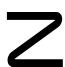
\includegraphics[keepaspectratio]{images/part001_3d6df7c1.jpg}}

The relation \([M:L]=0\) therefore means that there exists no direct factor submodule of M isomorphic to L. This does not exclude the existence of a submodule of M isomorphic to L; it suffices to consider the example where A=Z, L=Z/2Z, and M=Z/4Z: the Z-modules L and M are primordial and not isomorphic, so that \([M:L]=0\) and L is isomorphic to the submodule \(2Z/4Z\) of M.

\subsection{The Structure of Modules of Finite Length}

THEOREM 2 (Krull--Remak--Schmidt). --- Let A be a ring and M an A-module of finite length.

\begin{enumerate}
\def\labelenumi{\alph{enumi})}
\item
  There exists a finite family \((\mathrm{M}_i)_{i\in \mathrm{I}}\) of indecomposable submodules of M such that \(\mathrm{M} = \bigoplus_{i\in \mathrm{I}}\mathrm{M}_i\) , and the module M is semiprimordial.
\item
  Let \((\mathrm{M}_{i})_{i\in\mathrm{I}}\) and \((\mathrm{M}_{j}^{\prime})_{j\in\mathrm{J}}\) be two finite families of indecomposable submodules of M such that \(M=\bigoplus_{i\in I}M_{i}=\bigoplus_{j\in J}M_{j}^{\prime}\) . There exist a bijection \(\sigma\) from I to J and an automorphism u of M such that we have \(u(\mathrm{M}_{i})=\mathrm{M}_{\sigma(i)}^{\prime}\) for every \(i\in I\) .
\item
  Let \(\mathrm{N}\) be a direct factor submodule of \(\mathrm{M}\) , and let \((\mathrm{M}_i)_{i\in \mathrm{I}}\) be a finite family of indecomposable submodules of \(\mathrm{M}\) with direct sum \(\mathrm{M}\) . There exists a subset \(\mathrm{J}\) of \(\mathrm{I}\) such that \(\bigoplus_{i\in \mathrm{I - J}}\mathrm{M}_i\) is supplementary to \(\mathrm{N}\) . The module \(\mathrm{N}\) is isomorphic to \(\bigoplus_{j\in \mathrm{J}}\mathrm{M}_j\) .
\item
  Let \(\mathbf{N}\) be an A-module. If there exists an integer \(d > 0\) such that the modules \(\mathbf{M}^d\) and \(\mathbf{N}^d\) are isomorphic, then the modules \(\mathbf{M}\) and \(\mathbf{N}\) are isomorphic.
\item
  Let \(\mathrm{N}\) and \(\mathrm{P}\) be A-modules of finite length. If the modules \(\mathrm{M} \oplus \mathrm{P}\) and \(\mathrm{N} \oplus \mathrm{P}\) are isomorphic, then \(\mathrm{M}\) and \(\mathrm{N}\) are isomorphic.
\end{enumerate}

A module of finite length is both Artinian and Noetherian (VIII, p.~2, Proposition 1). Moreover, for a module of finite length, being indecomposable or primordial amounts to the same (VIII, p.~31, Proposition 4). Assertion a) then follows from Proposition 3 of VIII, p.~30. Assertions b), c), and e) follow from, respectively, Corollaries 2, 5, and 3 of Theorem 1 of VIII, p.~32. Finally, assertion d) follows from Corollary 4 of VIII, p.~35 because under the assumptions of d), the module N has finite length and is therefore semiprimordial by a).

THEOREM 3. --- Let K be a commutative field, A a K-algebra, and M and N modules of finite length. Let \(K'\) be a nonzero commutative K-algebra such that the \(\mathrm{A}_{(\mathrm{K}')}\) -modules \(\mathrm{M}_{(\mathrm{K}')}\) and \(\mathrm{N}_{(\mathrm{K}')}\) are isomorphic. Then the A-modules M and N are isomorphic.

\begin{enumerate}
\def\labelenumi{\alph{enumi})}
\item
  First, suppose that the algebra \(K'\) has finite degree d over K. Then the A-module \(\mathrm{M}_{(\mathrm{K}')}\) is isomorphic to \(M^{d}\) and the A-module \(\mathrm{N}_{(\mathrm{K}')}\) is isomorphic to \(\mathbf{N}^d\) , so that the A-modules \(\mathbf{M}^d\) and \(\mathbf{N}^d\) are isomorphic. By Theorem 2, d), the A-modules \(\mathbf{M}\) and \(\mathbf{N}\) are isomorphic.
\item
  Now, suppose that the K-algebra \(K'\) is generated by finitely many elements. Choose a maximal ideal m of \(K'\) , and set \(K'' = K'/m\) . By Hilbert's Nullstellensatz (VIII, p.~462, Corollary 1 of Theorem 1), \(K''\) is a finite-degree extension of K. By extension of scalars from \(K'\) to \(K''\) , we deduce from the \(A_{(K')}\) -linear isomorphism \(M_{(K')} \to N_{(K')}\) an \(A_{(K'')}\) -linear isomorphism \(M_{(K'')} \to N_{(K'')}\) . By part a) of the proof, the A-modules M and N are isomorphic.
\item
  Finally, let us treat the general case. Let \(u: \mathrm{M}_{(\mathrm{K}')} \to \mathrm{N}_{(\mathrm{K}')}\) be an isomorphism of \(\mathrm{A}_{(\mathrm{K}')}\) -modules and \(v: \mathrm{N}_{(\mathrm{K}')} \to \mathrm{M}_{(\mathrm{K}')}\) the inverse isomorphism. Denote by \(\mathcal{E}\) the set of K-subalgebras of \(\mathrm{K}'\) generated by finitely many elements. If E is such a subalgebra, then \(\mathrm{A}_{(\mathrm{E})}\) is identified with a subring of \(\mathrm{A}_{(\mathrm{K}')}\) , and \(\mathrm{M}_{(\mathrm{E})}\) and \(\mathrm{N}_{(\mathrm{E})}\) are identified with \(\mathrm{A}_{(\mathrm{E})}\) -submodules of \(\mathrm{M}_{(\mathrm{K}')}\) and \(\mathrm{N}_{(\mathrm{K}')}\) , respectively (II, §7, No.~7, p.~306); moreover, \(\mathrm{M}_{(\mathrm{K}')}\) and \(\mathrm{N}_{(\mathrm{K}')}\) are unions of right directed families \((\mathrm{M}_{(\mathrm{E})})_{\mathrm{E} \in \mathcal{E}}\) and \((\mathrm{N}_{(\mathrm{E})})_{\mathrm{E} \in \mathcal{E}}\) , respectively. The A-modules M and N are of finite length, hence finitely generated; let S be a finite generating subset of the A-module M and T a finite generating subset of the A-module N. There exists a K-algebra \(\mathrm{E} \in \mathcal{E}\) such that we have \(u(1 \otimes s) \in \mathrm{N}_{(\mathrm{E})}\) for every \(s \in \mathrm{S}\) and \(v(1 \otimes t) \in \mathrm{M}_{(\mathrm{E})}\) for every \(t \in \mathrm{T}\) . It follows by linearity that we have \(u(\mathrm{M}_{(\mathrm{E})}) \subset \mathrm{N}_{(\mathrm{E})}\) and \(v(\mathrm{N}_{(\mathrm{E})}) \subset \mathrm{M}_{(\mathrm{E})}\) . The maps \(u\) and \(v\) then induce inverse bijections from \(\mathrm{M}_{(\mathrm{E})}\) to \(\mathrm{N}_{(\mathrm{E})}\) and from \(\mathrm{N}_{(\mathrm{E})}\) to \(\mathrm{M}_{(\mathrm{E})}\) . These bijections are clearly \(\mathrm{A}_{(\mathrm{E})}\) -linear. Thus, the \(\mathrm{A}_{(\mathrm{E})}\) -modules \(\mathrm{M}_{(\mathrm{E})}\) and \(\mathrm{N}_{(\mathrm{E})}\) are isomorphic. By part b) of the proof, the A-modules M and N are isomorphic.
\end{enumerate}

Remark. --- Let E and F be two finite-dimensional vector spaces over a commutative field K, and let \(K'\) be an extension of K. Let u be an endomorphism of E and v an endomorphism of F, and let \(u_{(K')}\) and \(v_{(K')}\) be the endomorphisms of \(E_{(K')}\) and \(F_{(K')}\) obtained by extension of scalars. It follows from Corollaries 1 and 2 of VII, §5, No.~3, p.~32 that the endomorphisms u and v are similar if and only if the endomorphisms \(u_{(K')}\) and \(v_{(K')}\) are. This also follows from Theorem 3 above applied to the algebra A = K{[}X{]} and the A-modules \(M = E_u\) and \(N = F_v\) (VII, §5, No.~1, p.~29).

\BourbakiExercises{Exercises}

\begin{enumerate}
\def\labelenumi{\arabic{enumi})}
\tightlist
\item
  \begin{enumerate}
  \def\labelenumii{\alph{enumii})}
  \tightlist
  \item
    Give an example of a Noetherian module M such that every nonzero endomorphism of M is injective and that there exist nonzero nonbijective endomorphisms of M.
  \end{enumerate}
\end{enumerate}

\begin{enumerate}
\def\labelenumi{\alph{enumi})}
\setcounter{enumi}{1}
\tightlist
\item
  Give an example of an Artinian module M such that every nonzero endomorphism of M is surjective and that there exist nonzero nonbijective endomorphisms of M.
\end{enumerate}

\begin{enumerate}
\def\labelenumi{\arabic{enumi})}
\setcounter{enumi}{1}
\item
  Let \(\mathrm{A}\) be a ring in which every increasing sequence \((\mathfrak{a}_n)_{n\in \mathbf{N}}\) of two-sided ideals is stationary (for example, a left or right Noetherian ring). Prove that every surjective endomorphism of the ring \(\mathrm{A}\) is bijective.
\item
  Give an example of a ring that has two elements u, v such that uv = 1 and \(vu \neq 1\) . Prove that such a ring is not the union of a directed family of Noetherian subrings.
\item
  Let M be an A-module and p and q two projectors of M.
\end{enumerate}

\begin{enumerate}
\def\labelenumi{\alph{enumi})}
\item
  We have \(p(\mathrm{M}) \subset q(\mathrm{M})\) if and only if we have qp = p; the kernel \(\operatorname{Ker}(p)\) is contained in \(\operatorname{Ker}(q)\) if and only if we have qp = q.
\item
  The sum \(p + q\) is a projector if and only if we have pq = -qp. If \(p + q\) is a projector and if in M, the relation 2x = 0 implies x = 0, then we have pq = 0 and qp = 0.
\item
  Prove that the following properties are equivalent:
\end{enumerate}

\begin{enumerate}
\def\labelenumi{(\roman{enumi})}
\item
  We have \(pq = qp\) .
\item
  We have \(q(p(\mathbb{M})) \subset p(\mathbb{M})\) and \(q(\operatorname{Ker}(p)) \subset \operatorname{Ker}(p)\) .
\item
  There exists a sequence \((p_1, p_2, p_3, p_4)\) of pairwise orthogonal projectors of M such that \(p = p_1 + p_2\) , \(q = p_1 + p_3\) , and \(1_{\mathrm{M}} = p_1 + p_2 + p_3 + p_4\) .
\end{enumerate}

Such a sequence, when it exists, is unique: we have \(p_{1} = pq\) .

\begin{enumerate}
\def\labelenumi{\arabic{enumi})}
\setcounter{enumi}{4}
\tightlist
\item
  Let \(\mathrm{A}\) be a ring.
\end{enumerate}

\begin{enumerate}
\def\labelenumi{\alph{enumi})}
\item
  An element e of A is idempotent if and only if the mapping \(x \mapsto xe\) is a projector of the left A-module \(A_{s}\) (resp. the mapping \(x \mapsto ex\) is a projector of the right A-module \(A_{d}\) ).
\item
  Let \(e_{1}, e_{2}\) be idempotents in the ring A. Prove that the group \(\mathrm{Hom}_{\mathrm{A}}(\mathrm{Ae}_{1}, \mathrm{Ae}_{2})\) is isomorphic to \(e_{1}A \cap Ae_{2} = e_{1}Ae_{2}\) and that the ring \(\mathrm{End}_{\mathrm{A}}(\mathrm{Ae}_{1})\) is isomorphic to the ring \(e_{1}Ae_{1}\) .
\item
  Let \(e_1, e_2\) be idempotents in A. Prove that the following properties are equivalent:
\end{enumerate}

\begin{enumerate}
\def\labelenumi{(\roman{enumi})}
\item
  \(Ae_{1} = Ae_{2}.\)
\item
  \(e_{1}e_{2}=e_{1}\) and \(e_{2}e_{1}=e_{2}\) .
\item
  \((1 - e_{1})\mathrm{A} = (1 - e_{2})\mathrm{A}.\)
\end{enumerate}

When they are satisfied, there exists an invertible element \(a \in \mathrm{A}\) such that \(e_2 = ae_1a^{-1}\) .

\begin{enumerate}
\def\labelenumi{\alph{enumi})}
\setcounter{enumi}{3}
\tightlist
\item
  Let \(e_{1}, e_{2}\) be two idempotents in A. Prove that the following properties are equivalent:
\end{enumerate}

\begin{enumerate}
\def\labelenumi{(\roman{enumi})}
\item
  The left A-modules \(Ae_{1}\) and \(Ae_{2}\) are isomorphic.
\item
  The right A-modules \(e_1\mathrm{A}\) and \(e_2\mathrm{A}\) are isomorphic.
\item
  There exist elements \(x, y\) of \(A\) such that \(xy = e_1\) and \(yx = e_2\) .
\end{enumerate}

When they are satisfied, we say that \(e_{1}\) and \(e_{2}\) are equivalent idempotents.

\begin{enumerate}
\def\labelenumi{\alph{enumi})}
\setcounter{enumi}{4}
\tightlist
\item
  If idempotents in A are equivalent and belong to the center of A, then they are equal.
\end{enumerate}

\(f\) ) Let \((e_i)_{i\in \mathrm{I}}\) and \((f_{i})_{i\in \mathrm{I}}\) be finite families of idempotents in A such that \(e_i e_j = 0\) and \(f_{i} f_{j} = 0\) for \(i\in \mathrm{I}, j\in \mathrm{I}, i\neq j\) and that \(e_i\) is equivalent to \(f_{i}\) for every \(i\in \mathrm{I}\) . Then \(e = \sum_{i\in \mathrm{I}}e_i\) and \(f = \sum_{i\in \mathrm{I}}f_{i}\) are equivalent idempotents in A.

¶ 6) Let A be a ring and u and v two elements of A such that uv = 1 and vu ≠ 1. For i ≥ 1 and j ≥ 1, we set \(e_{ij} = v^{i-1}u^{j-1} - v^i u^j\) .

\begin{enumerate}
\def\labelenumi{\alph{enumi})}
\item
  Prove that we have \(e_{ij} \neq 0\) and \(e_{ij}e_{hk} = \delta_{jh}e_{ik}\) for \(i,j,k,h\) integers \(\geqslant 1\) .
\item
  Prove that the left ideals \(Ae_{ii}\) of A (for \(i \geqslant 1\) ) are nonzero, pairwise isomorphic as A-modules (use Exercise 5 d)), and that their sum is direct.
\item
  Prove that we have \(u(v + e_{1i}) = 1\) for every \(i \geqslant 1\) and \(e_{1i} \neq e_{1j}\) for \(i \geqslant 1, j \geqslant 1, i \neq j\) .
\item
  Let B be a ring that has the equivalent properties of Exercise 7 of VIII, p.~15, a). Deduce from the above that every left or right invertible element of B is invertible.
\end{enumerate}

\begin{enumerate}
\def\labelenumi{\arabic{enumi})}
\setcounter{enumi}{6}
\tightlist
\item
  Denote by A (resp. a) the set of rational fractions of the form \(\mathrm{P}/(\mathrm{X}^{2}+1)^{n}\) , where n is an integer \(\geqslant0\) and \(P\in \mathbf{Q}[X]\) is a polynomial of degree \(\leqslant2n\) (resp. \(\leqslant2n-1\) ). a) Prove that A is a subring of the field \(\mathbf{Q}(X)\) and that a is an ideal of the ring A. b) The A-modules \(a\oplus a\) and \(A\oplus A\) are isomorphic. The A-module a is projective and finitely generated but is not isomorphic to A.
\end{enumerate}

\begin{enumerate}
\def\labelenumi{\alph{enumi})}
\setcounter{enumi}{2}
\tightlist
\item
  There exists a quadratic extension \(\mathbf{K}\) of the field \(\mathbf{Q}\) such that the \(\mathrm{A}_{(\mathrm{K})}\) -modules \(\mathfrak{a}_{(\mathrm{K})}\) and \(\mathrm{A}_{(\mathrm{K})}\) are isomorphic.
\end{enumerate}

\begin{enumerate}
\def\labelenumi{\arabic{enumi})}
\setcounter{enumi}{7}
\item
  Let A be a left Artinian ring, and let M and N be two supplementary submodules in the A-module \(A_{s}^{n}\) . If M is a free A-module, then N is a free A-module.
\item
  Let A be a complete topological ring and m a two-sided ideal of A. Suppose that the ring A/m is a field, that every element of m is topologically nilpotent (Gen.~Top., III, §6, p.~317, Exercise 9), and that there exists a fundamental system of neighborhoods of 0 in A consisting of subgroups of the additive group of A. Then the ring A is local and m is its maximal ideal. In particular, for every prime p, the ring \(\mathbf{Z}_{p}\) of p-adic integers (V, §12, No.~3, p.~96) is local, and its maximal ideal is \(p\mathbf{Z}_{p}\) .
\end{enumerate}

¶ 10) Let p be a prime number, q a power of p, G a finite group of order q, and A a commutative ring. Let \((e_{g})\) be the canonical basis of the algebra A{[}G{]} of the group G over A.

\begin{enumerate}
\def\labelenumi{\alph{enumi})}
\item
  The set \(\mathfrak{a}\) of elements \(\sum a_{g}e_{g}\) of A{[}G{]} such that \(\sum a_{g} = 0\) is a two-sided ideal of A{[}G{]}. If the ring A is of characteristic \(p\) (V, §1, No.~2, p.~2), then we have \(x^{q} = 0\) for every \(x\in \mathfrak{a}\) (use induction on \(q\) ; if \(q\neq 1\) , choose an element \(h\) of order \(p\) of the center of G (I, §6, No.~5, p.~77, Corollary of Proposition 11) and deduce from the induction hypothesis that there exists a \(y\in \mathrm{A}[\mathrm{G}]\) such that \(x^{q / p} = (1 - e_h)y\) ).
\item
  Suppose that A is a local ring, with maximal ideal m, and that the field A/m is of characteristic p.~Prove that the ring A{[}G{]} is local and that its maximal ideal is the set of elements \(\sum a_{g}e_{g}\in A[G]\) such that \(\sum a_{g}\in m\) .
\end{enumerate}

(Let S be a simple A{[}G{]}-module; prove that S is annihilated by m and then, by applying Proposition 11 of I, §6, No.~5, p.~76, to the Z{[}G{]}-submodule generated by a nonzero element of S, that S contains an element invariant under G.)

\begin{enumerate}
\def\labelenumi{\arabic{enumi})}
\setcounter{enumi}{10}
\tightlist
\item
  Let p be a prime number, G a group that does not contain any elements of order p, A a commutative ring of characteristic p that does not contain any nonzero nilpotent elements, A{[}G{]} the algebra of G over A, and \((e_{g})\) the canonical basis of A{[}G{]} over A. Prove that the ring A{[}G{]} has no nonzero nil ideal (observe that if an element \(\sum a_{g}e_{g} \in A[G]\) is nilpotent, then we have \(a_{1} = 0\) ).
\end{enumerate}

¶ 12) Let K be a commutative field, E and F extensions of K, and A the ring \(E \otimes_{K} F\) .

\begin{enumerate}
\def\labelenumi{\alph{enumi})}
\tightlist
\item
  If E and F are transcendental extensions of K, then the ring A is not local. b) Suppose that E is an algebraic extension of K, and denote the separable closures of K in E and F, respectively, by \(E_{s}\) and \(F_{s}\) . The following properties are equivalent:
\end{enumerate}

\begin{enumerate}
\def\labelenumi{(\roman{enumi})}
\item
  The ring A is local.
\item
  The ring \(\mathrm{E}\otimes_{\mathrm{K}}\mathrm{F}_s\) is an integral domain.
\item
  The ring \(E \otimes_{K} F_{s}\) is a field.
\item
  The ring \(E_{s} \otimes_{K} F_{s}\) is a field.
\end{enumerate}

When they hold, the maximal ideal \(\mathfrak{m}\) of A is the set of nilpotent elements of A, and every composite extension of E and F is isomorphic to \(A / \mathfrak{m}\) .

\begin{enumerate}
\def\labelenumi{\arabic{enumi})}
\setcounter{enumi}{12}
\item
  Let A be a local integral domain that is not a field (for example \(\mathbf{Z}_{(p)}\) , cf.~VIII, p.~26, Example 5), and let a be a nonzero noninvertible element of A. Denote the A-module \(\mathrm{A}^{(\mathbf{N})}\) by M and its canonical basis by \((e_{n})_{n\in\mathbf{N}}\) . Prove that the sequence \((f_{n})_{n\in\mathbf{N}}\) , where \(f_{2m}=e_{2m}\) and \(f_{2m+1}=e_{2m+1}+ae_{2m+2}\) for every \(m\geqslant0\) , is a basis of M over A. Prove that the submodule \(N=\sum_{m\geqslant0}\mathrm{A}(e_{2m}+ae_{2m+1})\) of M is a direct factor but that there is no subset J of N such that \(\sum_{n\in J}Af_{j}\) is supplementary to N. Deduce that in Corollary 5 of VIII, p.~35, we cannot leave out the assumption that I is finite.
\item
  Let A be a ring, M an A-module, and N a primordial direct factor of M. Let \(M = \bigoplus_{i \in I} M_i\) be a decomposition of M into a direct sum, and let \((p_i)_{i \in I}\) be the associated family of projectors. Prove that there exists an \(i \in I\) such that \(p_i\) induces an isomorphism from N to a direct factor of \(M_i\) .
\item
  Let A be a ring, and let M, N, P be A-modules. If the modules \(M \oplus P\) and \(N \oplus P\) are isomorphic and the module P is primordial, then the modules M and N are isomorphic.
\item
  Let A be a ring, M an A-module of finite length, and \((\mathrm{M}_{i})_{i\in\mathrm{I}}\) a family of indecomposable submodules of M with direct sum M. Let L be an indecomposable A-module of finite length and \(I_{L}\) the set of indices \(i\in I\) such that \(M_{i}\) is isomorphic to L. Use an example to show that the submodule \(\sum_{i\in I_{L}}M_{i}\) of M is not necessarily stable under the automorphisms of M.
\item
  Let \(\mathrm{A}\) be a ring, \(n\) an integer, and \(X \in \mathbf{GL}_n(\mathrm{A})\) .
\end{enumerate}

\begin{enumerate}
\def\labelenumi{\alph{enumi})}
\item
  Suppose that the ring A is local. Prove that there exist matrices P, Q in \(\mathbf{GL}_{n}(\mathrm{A})\) that are products of matrices of the form \(B_{ij}(\lambda)\) (II, §10, No.~13, p.~361) and an invertible element \(\delta\) of A, such that we have \(PXQ = \text{diag}(1, \ldots, 1, \delta)\) (follow the proof of Proposition 14 of loc. cit.).
\item
  Suppose that the ring A is Euclidean (VII, §1, p.~49, Exercise 7). Prove the same result.
\item
  If \(\mathrm{A}\) is a local ring or a Euclidean commutative ring, then the group \(\mathbf{S}\mathbf{L}_n(\mathbf{A})\) is generated by the matrices \(B_{ij}(\lambda)\) .
\item
  Suppose that A is local, and denote its maximal ideal by m. Prove that every matrix in \(\mathbf{M}_{n}(\mathrm{A})\) with invertible image in \(\mathbf{M}_{n}(\mathrm{A}/\mathfrak{m})\) is itself invertible (use Lemma 1 of II, §10, No.~13, p.~361).
\end{enumerate}

\begin{enumerate}
\def\labelenumi{\arabic{enumi})}
\setcounter{enumi}{17}
\tightlist
\item
  Let A be a local ring, E a free A-module, and x a nonzero element of E. Let \((e_{i})_{i\in I}\) be a basis of E in which the number of nonzero coordinates of x is the least possible. Let \(x=\sum a_{i}e_{i}\) be the representation of x in this basis; denote the set of indices \(i\in I\) such that \(a_{i}\neq0\) by J.
\end{enumerate}

\begin{enumerate}
\def\labelenumi{\alph{enumi})}
\tightlist
\item
  Prove that none of the \(a_{i}\) belong to the right ideal of A generated by the others.
\item
  Let F and G be supplementary submodules of E such that \(x \in F\) ; for \(i \in I\) , write \(e_{i} = f_{i} + g_{i}\) with \(f_{i} \in F\) and \(g_{i} \in G\) . Prove that the family consisting of the \(f_{j}\) for \(j \in J\) and the \(e_{i}\) for \(i \in I - J\) is a basis of E (if \(g_{j} = \sum_{k \in I} b_{jk} e_{k}\) , observe that the coordinates \(b_{jk}\) for j, k in J belong to the maximal ideal of A, and apply Exercise 17 d)). Deduce that there exists a free submodule of F that contains x and is a direct factor of F.
\end{enumerate}

\(c\) ) Prove that every projective A-module is free (use Kaplansky's theorem (II, §2, p.~386, Exercise 2) to reduce to the case of a module with a countable family of generators, and apply \(b\) )).

\begin{enumerate}
\def\labelenumi{\arabic{enumi})}
\setcounter{enumi}{18}
\item
  Let A be a commutative ring, M a finitely generated A-module, u an automorphism of M, and N a submodule of M that is stable under u. Prove that we have \(u(N) = N\) (use Corollary 1, d) of VIII, p.~28).
\item
  Let A be ring, let M be an A-module of finite length, and let N be an A-module. Let m and n be strictly positive integers such that \(M^{m}\) and \(N^{n}\) are isomorphic. Prove that there exist an A-module P and integers p, q such that M is isomorphic to \(P^{p}\) , N is isomorphic to \(P^{q}\) , and mp = nq.
\end{enumerate}

\section{Simple Modules}

\subsection{Simple Modules}

Recall the following definition (II, §1, No.~10, p.~212).

DEFINITION 1. --- Let A be a ring. An A-module M is called simple if it is nonzero and has no submodule distinct from 0 and M.

An A-module M is simple if and only if M is a simple module over its ring of homotheties \(A_{M}\) . Every simple module is indecomposable, of length 1, and therefore primordial (VIII, p.~31, Proposition 4, b)).

Examples. --- 1) The module \(A_{s}\) is a simple A-module if and only if A is a field (I, §9, No.~1, p.~115, Theorem 1). The simple A-modules are then the vector spaces of dimension 1 over the field A.

\begin{enumerate}
\def\labelenumi{\arabic{enumi})}
\setcounter{enumi}{1}
\item
  Let A be a principal ideal domain (VII, §1, No.~1, p.~1, Definition 1) that is not a field. For every irreducible element \(\pi\) of A, the A-module \(A_s / (\pi)\) is simple, and every simple A-module is isomorphic to such a module (VII, §4, No.~8, p.~25, Remark 4). For \(n \geqslant 2\) , the A-module \(A_s / (\pi^n)\) is indecomposable (VII, §4, No.~8, p.~24, Proposition 8) but not simple.
\item
  Let K be a field, V a nonzero right vector space over the field K, and A a subring of the ring \(\operatorname{End}_{\mathrm{K}}(\mathrm{V})\) containing the endomorphisms of V of finite rank (for example, \(\mathrm{A} = \operatorname{End}_{\mathrm{K}}(\mathrm{V})\) ). Let us prove that V is a simple A-module: let W be a nonzero A-submodule of V and x a nonzero element of W; there exists a linear form \(\varphi\) on V such that \(\varphi(x) \neq 0\) (II, §7, No.~5, p.~300, Theorem 6). For every y in V, the mapping \(z \mapsto y\varphi(z)\) , which is linear of rank \(\leqslant 1\) , belongs to A; we therefore have Ax = V, hence a fortiori W = V, which proves that V is a simple A-module.
\end{enumerate}

PROPOSITION 1. --- Let A be a ring.

\begin{enumerate}
\def\labelenumi{\alph{enumi})}
\item
  Let \(\mathfrak{m}\) be a left ideal of A. The A-module \(\mathrm{A}_s / \mathfrak{m}\) is simple if and only if \(\mathfrak{m}\) is a maximal left ideal.
\item
  Let M be a simple A-module, and let x be a nonzero element of M. We have the equality \(M = Ax\) , the annihilator m of x is a maximal left ideal of A, and the mapping \(a \mapsto ax\) defines, by passing to the quotient, an isomorphism from \(A_{s}/m\) to M.
\item
  Let M be a nonzero A-module. If we have M = Ax for every nonzero element x of M, then M is simple.
\end{enumerate}

The submodules of \(A_{s}/m\) are of the form n/m, where n is a left ideal of A containing m (I, §4, No.~6, p.~41, Theorem 4); consequently, the A-module \(A_{s}/m\) is simple if and only if we have \(m \neq A\) and every left ideal n of A containing m satisfies n/m = 0 or \(n/m = A_{s}/m\) , that is, n = m or n = A. This proves a).

Under the assumptions of b), Ax is a nonzero submodule of M, hence is equal to M. Consequently, the mapping \(a \mapsto ax\) defines, by passing to the quotient, an isomorphism from \(A_{s}/m\) to M; the A-module \(A_{s}/m\) is therefore simple, and the left ideal m is maximal by a). This proves b).

Under the assumptions of c), let N be a nonzero submodule of M. If x is a nonzero element of N, then we have \(Ax \subset N\) and Ax = M, and therefore M = N. Hence M is simple.

COROLLARY 1. --- If the ring A is not reduced to 0, then there exist simple A-modules.

Indeed, by Krull's theorem (I, §8, No.~6, p.~104, Theorem 1), there exist maximal left ideals of A.

COROLLARY 2. --- Let A be a local ring (VIII, p.~26, Definition 1) and r its maximal ideal. The A-module \(A_{s}/r\) is simple, and every simple A-module is isomorphic to \(A_{s}/r\) .

Remarks. --- 1) Let A be a commutative ring and m an ideal of A. Then m is the annihilator (II, §1, No.~12, p.~219, Definition 11) of the A-module \(A_{s}/m\) . Hence, if m and \(m'\) are distinct ideals of A, then the A-modules \(A_{s}/m\) and \(A_{s}/m'\) are not isomorphic. There exists a faithful simple A-module (II, §1, No.~12, p.~219) if and only if (0) is a maximal ideal of A, that is, A is a field.

\begin{enumerate}
\def\labelenumi{\arabic{enumi})}
\setcounter{enumi}{1}
\tightlist
\item
  We can give an example of a noncommutative ring A and two distinct maximal left ideals m and \(m'\) of A such that the A-modules \(A_{s}/m\) and \(A_{s}/m'\) are isomorphic (VIII, p.~52, Exercise 3).
\end{enumerate}

\subsection{Schur's Lemma}

PROPOSITION 2. --- Let A be a ring, M and N two A-modules, and f a nonzero homomorphism from M to N.

\begin{enumerate}
\def\labelenumi{\alph{enumi})}
\item
  If M is simple, then f is injective.
\item
  If \(\mathbf{N}\) is simple, then \(f\) is surjective.
\item
  If M and N are simple, then f is an isomorphism.
\end{enumerate}

The kernel of f is a proper submodule of M, and the image of f is a nonzero submodule of N.

\begin{enumerate}
\def\labelenumi{\alph{enumi})}
\item
  If M is simple, then we have \(\operatorname{Ker}(f)=0\) , so f is injective.
\item
  If \(N\) is simple, then we have \(\operatorname{Im}(f) = N\) , so \(f\) is surjective.
\item
  If M and N are simple, then f is both injective and surjective.
\end{enumerate}

COROLLARY (Schur's lemma). --- The endomorphism ring of a simple module is a field.

If M is a simple A-module, then every nonzero element of the nonzero ring \(\operatorname{End}_{\mathrm{A}}(\mathrm{M})\) is invertible (Proposition 2, c)), so \(\operatorname{End}_{\mathrm{A}}(\mathrm{M})\) is a field.

THEOREM 1. --- Let K be an algebraically closed commutative field, A a K-algebra, and M a simple A-module. Suppose that the dimension of M as a vector space over K is finite or, more generally, strictly less than the cardinal of K. Then the endomorphism ring of the A-module M consists of the homotheties \(\alpha_{M}\) with \(\alpha \in K\) .

Let \(\mathrm{E}\) be the endomorphism ring of the A-module \(\mathrm{M}\) ; it is a field by the corollary of Proposition 2 and an algebra over the field \(\mathrm{K}\) . If we view \(\mathrm{M}\) as a left vector space over the field \(\mathrm{E}\) , then we have \(\dim_{\mathrm{K}} \mathrm{M} = (\dim_{\mathrm{E}} \mathrm{M})[\mathrm{E} : \mathrm{K}]\) by Proposition 25 of II, §1, No.~13, p.~222, hence \(\dim_{\mathrm{K}} \mathrm{M} \geqslant [\mathrm{E} : \mathrm{K}]\) . Since \(\dim_{\mathrm{K}} \mathrm{M} < \operatorname{Card}(\mathrm{K})\) by assumption, the equality \(\mathrm{E} = \mathrm{K} \cdot 1_{\mathrm{M}}\) is then a consequence of the following lemma.

Lemma 1. --- Let E be a field and K a subfield of the center of E not equal to E. If the field K is algebraically closed, then we have \([E:K] \geqslant \text{Card}(K)\) .

Let \(x\) be an element of \(\mathrm{E} - \mathrm{K}\) and \(\mathrm{L}\) the (commutative) subfield of \(\mathrm{E}\) generated by \(\mathrm{K} \cup \{x\}\) . Since \(\mathrm{K}\) is algebraically closed, \(x\) is transcendent over \(\mathrm{K}\) . By VII, §2, No.~3, p.~10, Theorem 2 and p.~11, the elements \((x - \alpha)^{-1}\) of \(\mathrm{L}\) , where \(\alpha\) runs through \(\mathrm{K}\) , are linearly independent over \(\mathrm{K}\) . We therefore have \([\mathrm{E} : \mathrm{K}] \geqslant [\mathrm{L} : \mathrm{K}] \geqslant \operatorname{Card}(\mathrm{K})\) .

Example. --- *Let A be a C-algebra generated by a countable family of elements; it has countable dimension over C. Let M be a simple A-module;

it is monogenous, so admits a countable basis over \(\mathbf{C}\) . Since the field \(\mathbf{C}\) is not countable (Gen.~Top., IV, §4, No.~1, p.~44), we have \([\mathrm{M}:\mathbf{C}] < \mathrm{Card}(\mathbf{C})\) . Therefore the endomorphisms of the A-module M are the homotheties \(\alpha_{\mathrm{M}}\) with \(\alpha \in \mathbf{C}\) . This applies, in particular, when A is the universal enveloping algebra of a finite-dimensional Lie algebra over \(\mathbf{C}\) (Lie, I, §2, No.~7, p.~21, Corollary 3).*

COROLLARY 1. --- Keep the assumptions of Theorem 1, and suppose, moreover, that the algebra A is commutative. Then M has dimension 1 over K.

Since the ring A is commutative, \(a_{M}\) is an endomorphism of the A-module M for every \(a \in A\) . By Theorem 1, we therefore have \(A_{M} = K \cdot 1_{M}\) , and M is a simple K-module, that is, a 1-dimensional vector space over the field K.

COROLLARY 2. --- Let K be a commutative field, A a K-algebra, and M an A-module. Suppose that for every extension L of K, the \(\mathrm{A}_{(\mathrm{L})}\) -module \(\mathrm{M}_{(\mathrm{L})}\) is simple. Then the endomorphism ring of M consists of the homotheties \(\alpha_{M}\) with \(\alpha \in K\) .

Let I be a set of cardinal strictly greater than the dimension of M over K (for example, the set of subsets of M). Let L be an algebraic closure of the field \(\mathrm{K}((\mathrm{X}_{i})_{i\in\mathrm{I}})\) (V, §4, No.~3, p.~23, Theorem 2). Choose a K-linear form \(\varphi\) on L such that \(\varphi(1)=1\) , and let \(v:M_{(\mathrm{L})}\to M\) be the K-linear mapping characterized by \(v(\alpha\otimes m)=\varphi(\alpha)m\) . Let u be an endomorphism of M. The dimension of \(M_{(\mathrm{L})}\) over L is equal to that of M over K and is strictly less than the cardinal of L. By Theorem 1, the endomorphism \(1_{L}\otimes u\) of the \(A_{(\mathrm{L})}\) -module \(M_{(\mathrm{L})}\) is of the form \(\lambda\otimes1_{M}\) with \(\lambda\in L\) . For every \(x\in M\) , we have

\[
\begin{array}{c} u (x) = v \bigl (1 \otimes u (x) \bigr) = v \bigl ((1 _ {\mathrm{L}} \otimes u) (1 \otimes x) \bigr) \\ = v \bigl ((\lambda \otimes 1 _ {\mathrm{M}}) (1 \otimes x) \bigr) = v (\lambda \otimes x) = \varphi (\lambda) x, \end{array}
\]

so that u is the homothety \(\varphi(\lambda)_{\mathrm{M}}\) .

\subsection{Maximal Submodules}

DEFINITION 2. --- Let A be a ring and M an A-module. A maximal submodule of M is a maximal element, for the inclusion, of the set of proper submodules of M.

A maximal submodule of \(A_{s}\) is simply a left maximal ideal of A.

Let N be a submodule of M. The submodules of M/N are of the form P/N, where P is a submodule of M containing N (I, §4, No.~6, p.~41, Theorem 4). Consequently, N is a maximal submodule of M if and only if the module M/N is simple.

PROPOSITION 3. --- Let M be a finitely generated A-module. Every proper submodule of M is contained in a maximal submodule.

Let N be a proper submodule of M. Denote by S the set of proper submodules of M containing N, ordered by inclusion; let us prove that S is inductive. Let F be a totally ordered subset of S. If F is empty, then N is an upper bound for F in S. In the opposite case, denote by Q the union of the elements of F. Then Q is a submodule of M. Let F be a finite generating subset of M. If Q were equal to M, then F would be contained in a submodule \(P \in F\) , which would imply P = M, contrary to the definition of F. We therefore have \(Q \in S\) , which proves that S is inductive. Proposition 3 then follows from Corollary 1 of Set Theory, III, §2, No.~4, p.~155.

COROLLARY 1. --- Let M be a nonzero finitely generated A-module. There exists a two-sided ideal a of A, annihilator of a simple A-module, such that aM is not equal to M.

Let N be a maximal submodule of M (Proposition 3), and let a be the annihilator of the simple A-module M/N; it is a two-sided ideal of A, and we have \(\mathfrak{a}(M/N)=0\) , whence \(aM\subset N\) and consequently \(aM\neq M\) .

COROLLARY 2. --- Let A be a commutative ring and B an A-algebra. Let M be a simple B-module that is a finitely generated A-module, and let m be the annihilator of the A-module M. Then m is a maximal ideal of A, and M is a finite-dimensional vector space over the field A/m.

Since the ring A is commutative, the annihilator of a simple A-module is a maximal ideal of A (VIII, p.~46, Proposition 1). By Corollary 1 applied to the A-module M, there exists a maximal ideal a of A such that \(aM \neq M\) . But aM is a submodule of the simple B-module M; we therefore have aM = 0 and consequently \(a \subset m\) . Since the ideal m is distinct from A, it is equal to a, so that m is maximal. The module M is a finitely generated module over the field A/m; the last assertion follows.

\subsection{Simple Modules over an Artinian Ring}

Let A be a ring. By abuse of language, we say that a left ideal \(\alpha\) is a minimal left ideal of A if it is a minimal element of the set of nonzero left ideals of A, ordered by inclusion. We define right minimal ideals and two-sided minimal ideals analogously.

Let \(\mathfrak{a}\) be a left ideal of A. Then \(\mathfrak{a}\) is a simple A-module if and only if it is a minimal left ideal of A.

Every nonzero left ideal of a left Artinian (VIII, p.~1, Definition 1) ring contains a minimal left ideal.

PROPOSITION 4. --- Let A be a ring that has a minimal left ideal a. Every faithful simple A-module is isomorphic to the A-module a.

Let M be a faithful simple A-module. Let \(\alpha\) be a nonzero element of a. Since the A-module M is faithful, there exists an element x of M such that \(\alpha x \neq 0\) . The homomorphism \(a \mapsto ax\) from a to M is then nonzero; it is therefore an isomorphism by Proposition 2 of VIII, p.~47.

PROPOSITION 5. --- Let A be a left Artinian ring and M a faithful A-module.

\begin{enumerate}
\def\labelenumi{\alph{enumi})}
\item
  There exist a natural number \(m\) and an isomorphism from \(\mathbf{A}_s\) to a submodule of \(\mathbf{M}^m\) .
\item
  If M admits a Jordan--Hölder series \((\mathrm{M}_{i})_{0\leqslant i\leqslant n}\) , then every simple A-module is isomorphic to one of the quotients \(M_{i}/M_{i+1}\) .
\end{enumerate}

By VIII, p.~2 applied to the A-module \(A_{s}\) and the annihilators of the elements of M, there exist elements \(x_{1},\ldots,x_{m}\) of M such that the annihilator of M is the intersection of the annihilators of the \(x_{i}\) . Since the A-module M is faithful, the A-linear mapping \(a\mapsto(ax_{1},\ldots,ax_{m})\) from \(A_{s}\) to \(M^{m}\) is injective, whence a).

Under the assumption of b), every simple quotient of \(A_{s}\) is isomorphic to a quotient of a Jordan--Hölder series of \(M^{m}\) (I, §4, No.~7, p.~43, Corollary), hence to one of the modules \(M_{i}/M_{i+1}\) (I, §4, No.~7, p.~43, Theorem 6). We conclude that every simple A-module is isomorphic to a quotient of \(A_{s}\) .

Remark. --- Proposition 5 applies, in particular, to the following two cases:

\begin{enumerate}
\def\labelenumi{\alph{enumi})}
\item
  Let A be an algebra over a commutative field K, and let M be a faithful finite-dimensional module over K. Then M is an A-module of finite length, and the countermodule of M is finitely generated. The ring A is left Artinian (VIII, p.~9, Proposition 6). There exists a Jordan--Hölder series \((\mathrm{M}_{i})_{0\leqslant i\leqslant n}\) of the A-module M, and every simple A-module is isomorphic to one of the modules \(M_{i}/M_{i+1}\) for \(0\leqslant i\leqslant n-1\) .
\item
  Let A be a left Artinian ring. The module \(A_{s}\) has finite length (VIII, p.~6, Theorem 1). Since the A-module \(A_{s}\) has finite length, there exists a decreasing sequence \((\mathfrak{a}_{i})_{0\leqslant i\leqslant n}\) of left ideals of A such that \(a_{0}=A\) and \(a_{n}=0\) and that the A-modules \(S_{i}=\mathfrak{a}_{i-1}/\mathfrak{a}_{i}\) are simple for \(1\leqslant i\leqslant n\) . Then every simple A-module is isomorphic to one of the modules \(S_{1},\ldots,S_{n}\) .
\end{enumerate}

\subsection{Classes of Simple Modules}

Denote by \(\mathrm{Is}_{\mathrm{A}}\{\mathrm{X},\mathrm{Y}\}\) the relation

``A is a ring and X, Y are isomorphic A-modules.''

This is an equivalence relation with respect to X and Y. If X is an A-module, then we denote the class of objects equivalent to X for \(\operatorname{Is}_{\mathrm{A}}\) by \(\operatorname{cl}(\mathrm{X})\) and call it the class of the A-module X (Set Theory, II, §6, No.~9, p.~122). By definition, \(\operatorname{cl}(\mathrm{X})\) is an A-module isomorphic to X; moreover, two A-modules X and Y are isomorphic if and only if we have \(\operatorname{cl}(\mathrm{X}) = \operatorname{cl}(\mathrm{Y})\) .

Let A be a ring. The relation

``\(\lambda\) is a class of finitely generated A-modules''

is collectivizing in \(\lambda\) (Set Theory, II, §1, No.~4, p.~68). Indeed, every finitely generated A-module is isomorphic to an A-module of the form \(A_{s}^{n}/R\) , where n is a natural number and R a submodule of \(A_{s}^{n}\) , so that our assertion follows from Set Theory, II, §6, No.~9, p.~122.

We denote the set of classes of finitely generated A-modules by \(\mathcal{F}(A)\) . Every simple A-module is monogenous (VIII, p.~46, Proposition 1), and consequently the classes of the simple A-modules form a subset of \(\mathcal{F}(A)\) , which we from now on denote by \(\mathcal{S}(A)\) (or simply S). When the ring A is commutative, the mapping \(\mathfrak{m} \mapsto \operatorname{cl}(A/\mathfrak{m})\) is a bijection from the set of maximal ideals of A to the set \(\mathcal{S}(A)\) (loc. cit. and VIII, p.~46, Remark 1). When A is left Artinian, the set \(\mathcal{S}(A)\) is finite (VIII, p.~51, Remark b)).

\BourbakiExercises{Exercises}

\begin{enumerate}
\def\labelenumi{\arabic{enumi})}
\item
  Let A be a ring and m a maximal left ideal of A. Let B be the set of elements b of A such that \(mb \subset m\) . Prove that B is the largest subring of A containing m in which m is a two-sided ideal. Let S be the A-module \(A_{s}/m\) , D its commutant, and \(\pi\) the canonical mapping from \(A_{s}\) to S. Prove that, given \(b \in B\) , there exists a unique element \(u_{b}\) of \(\operatorname{End}_{\mathrm{A}}(\mathrm{S})\) such that \(u_{b}(\pi(a)) = \pi(ab)\) for every \(a \in A\) . The mapping \(b \mapsto u_{b}\) induces an isomorphism from B/m to \(\operatorname{End}_{\mathrm{A}}(\mathrm{S})\) .
\item
  Let D be a field, V a right D-vector space, and A a subring of \(\operatorname{End}_{\mathrm{D}}(\mathrm{V})\) that contains the endomorphisms of finite rank (for example, \(A = \operatorname{End}_{\mathrm{D}}(\mathrm{V})\) ). Prove that the dual \(V^{*} = \operatorname{Hom}_{\mathrm{D}}(\mathrm{V}, \mathrm{D})\) is simple as a right A-module.
\item
  Let D be a field, V a right D-vector space, and A the endomorphism ring of V. For every line L in V, we denote by \(m_{L}\) the set of elements u of A such that \(u(L)=0\) . Prove that \(m_{L}\) is a maximal ideal of A, that we have \(m_{L}\neq m_{L'}\) for \(L\neq L'\) , but that the simple A-modules \(A/m_{L}\) are all isomorphic to the A-module V.
\item
  Prove that the Z-module Q admits neither a simple submodule nor a simple quotient module.
\item
  Let \(\mathrm{A}\) be a ring.
\end{enumerate}

\begin{enumerate}
\def\labelenumi{\alph{enumi})}
\tightlist
\item
  Let M, N be monogenous A-modules. Prove that the following properties are equivalent:
\end{enumerate}

\begin{enumerate}
\def\labelenumi{(\roman{enumi})}
\item
  The A-modules M and N are isomorphic.
\item
  For every generator \(m\) of \(\mathrm{M}\) , there exists a generator \(n\) of \(\mathrm{N}\) that has the same annihilator as \(m\) .
\item
  There exist a generator of M and a generator of N that have the same annihilator.
\end{enumerate}

\begin{enumerate}
\def\labelenumi{\alph{enumi})}
\setcounter{enumi}{1}
\item
  Let \(\mathfrak{a},\mathfrak{b}\) be (left) ideals of A. The A-modules A/ \(\mathfrak{a}\) and A/ \(\mathfrak{b}\) are isomorphic if and only if there exists an element \(a\) of A such that \(Aa + \mathfrak{b} = A\) and \(\mathfrak{a}\) is the set of elements \(x\) of A such that \(xa\in \mathfrak{b}\) (use \(a\) ).
\item
  Let \(\mathfrak{m}\) and \(\mathfrak{n}\) be maximal left ideals of A. The simple A-modules A/ \(\mathfrak{m}\) and A/ \(\mathfrak{n}\) are isomorphic if and only if there exists an element \(a\) of A- \(\mathfrak{n}\) such that \(\mathfrak{ma} \subset \mathfrak{n}\) . d) Deduce from b) that the set of quotient A-modules of the A-module \(\mathrm{A}_s\) isomorphic to a given module has cardinal less than \(\operatorname{Card}(\mathrm{A})\) .
\end{enumerate}

\begin{enumerate}
\def\labelenumi{\arabic{enumi})}
\setcounter{enumi}{5}
\item
  Let M be an A-module such that for every \(x \neq 0\) in M, the module Ax is simple. Prove that either M is simple, or the ring of homotheties \(A_{M}\) is a field (if M is not simple, consider two nonzero elements x, y of M such that \(y \notin Ax\) and the annihilator of \(x + y\) ).
\item
  Let S be a simple A-module whose dual \(S^{*}\) and bidual \(S^{**}\) are simple. Prove that the mapping \(u \mapsto {}^{t}u\) is an isomorphism from \(\operatorname{End}_{\mathrm{A}}(\mathrm{S})\) to the opposite field of \(\operatorname{End}_{\mathrm{A}}(\mathrm{S}^{*})\) .
\end{enumerate}

¶ 8) Let A be a ring such that the A-modules \(A_{s}\) and \(A_{d}\) are of finite length. We identify \(A_{d}\) with the dual of \(A_{s}\) . For every left ideal s of A, the orthogonal \(s^{0}\) of s is the right annihilator of s in A; likewise, for every right ideal d, the orthogonal \(d^{0}\) is the left annihilator of d.~Prove that the following properties are equivalent:

\begin{enumerate}
\def\labelenumi{(\roman{enumi})}
\item
  Every simple (left or right) A-module is reflexive.
\item
  The dual of any (left or right) simple A-module is simple.
\item
  For every minimal left ideal \(\mathfrak{s}\) and every minimal right ideal \(\mathfrak{d}\) , we have \(\mathfrak{s}^{00} = \mathfrak{s}\) and \(\mathfrak{d}^{00} = \mathfrak{d}\) .
\item
  The mapping \(\mathfrak{s} \mapsto \mathfrak{s}^0\) is a bijection from the set of left ideals of \(A\) to the set of right ideals.
\end{enumerate}

When these properties hold, we say that the ring A is autoinjective (cf.~X, §1, p.~171, exercice 26).

\begin{enumerate}
\def\labelenumi{\alph{enumi})}
\tightlist
\item
  Suppose that A is autoinjective; let M be a finitely generated (left or right) A-module. Prove that the following properties hold:
\end{enumerate}

(i') The A-module M is reflexive.

(ii') The length of \(\mathbf{M}^*\) is equal to that of \(\mathbf{M}\) .

(iii') For every submodule \(\mathrm{N}\) of \(\mathrm{M}\) , we have \(\mathrm{N}^{00} = \mathrm{N}\) .

(iv') The mapping \(N \mapsto N^{0}\) is a bijection from the set of submodules of M to the set of submodules of \(M^{*}\) .

\begin{enumerate}
\def\labelenumi{\arabic{enumi})}
\setcounter{enumi}{8}
\tightlist
\item
  The colength of a simple A-module S is the dimension of the countermodule of S (over the field \(\operatorname{End}_{\mathrm{A}}(\mathrm{S})\) ). We say that an A-module M of finite length has finite colength if it admits a Jordan--Hölder series whose successive quotients are of finite colength; the sum of these colengths is called the colength of M and is denoted by \(\lambda(\mathrm{M})\) . If N is a submodule of M, then we have \(\lambda(\mathrm{M}) = \lambda(\mathrm{N}) + \lambda(\mathrm{M}/\mathrm{N})\) .
\end{enumerate}

Let A be an autoinjective ring (Exercise 8) such that the modules \(A_{s}\) and \(A_{d}\) are of finite colength. We say that A is a Frobenius ring if for every simple A-module S, we have \(\lambda(S) = \lambda(S^{*})\) .

\begin{enumerate}
\def\labelenumi{\alph{enumi})}
\item
  Let M be an A-module of finite length. If A is a Frobenius ring, then we have \(\lambda(M) = \lambda(M^{*})\) . If, moreover, A is an algebra of finite rank over a commutative field K, then we have \(\dim_K(M) = \dim_K(M^*)\) (use Exercise 7).
\item
  Let K be a commutative field, and let A be the subalgebra of \(\mathbf{M}_{6}(\mathrm{K})\) with basis the elements \(E_{11} + E_{55}\) , \(E_{12} + E_{56}\) , \(E_{21} + E_{65}\) , \(E_{22} + E_{66}\) , \(E_{33} + E_{44}\) , \(E_{13}\) , \(E_{23}\) , \(E_{45}\) , and \(E_{46}\) (where the \(E_{ij}\) are the matrix units of \(\mathbf{M}_{6}(\mathrm{K})\) ). Prove that A is an autoinjective algebra but not a Frobenius algebra (observe that the minimal left ideals of A are \(KE_{13} + KE_{23}\) , \(KE_{45}\) , and \(KE_{46}\) , and the minimal right ideals are \(KE_{13}\) , \(KE_{23}\) , and \(KE_{45} + KE_{46}\) ).
\end{enumerate}

\begin{enumerate}
\def\labelenumi{\arabic{enumi})}
\setcounter{enumi}{9}
\tightlist
\item
  Let \(\rho : \mathrm{A} \to \mathrm{B}\) be a ring homomorphism used to view B as a right A-module. Suppose that the left B-module \(\operatorname{Hom}_{\mathrm{A}}(\mathrm{B}, \mathrm{A})\) is isomorphic to \(\mathrm{B}_s\) .
\end{enumerate}

\begin{enumerate}
\def\labelenumi{\alph{enumi})}
\item
  Let M be a B-module, and let \(\varphi : \mathrm{B}_s \to \mathrm{Hom}_{\mathrm{A}}(\mathrm{B}, \mathrm{A})\) be an isomorphism. Prove that the mapping \(u \mapsto \varphi(1) \circ u\) from \(\mathrm{Hom}_{\mathrm{B}}(\mathrm{M}, \mathrm{B})\) to \(\mathrm{Hom}_{\mathrm{A}}(\mathrm{M}, \mathrm{A})\) is bijective.
\item
  Suppose, moreover, that the A-module B is finitely generated. The ring B is autoinjective (Exercise 8) if and only if the same holds for A.
\item
  Let G be a finite group. Show that the conditions above are satisfied when B is taken to be the A-module A{[}G{]} endowed with the ring structure such that \((ae_{g})(a^{\prime}e_{g^{\prime}})=aa^{\prime}e_{gg^{\prime}}\) for \(a,a^{\prime}\) in A and \(g,g^{\prime}\) in G. In particular, if K is a commutative field, then the algebra K{[}G{]} is autoinjective.
\end{enumerate}

\section{Semisimple Modules}

\subsection{Semisimple Modules}

DEFINITION 1. --- A module is called semisimple if it is the direct sum of a family of simple modules. \(^{(1)}\) .

A multimodule is called semisimple if it is the direct sum of a family of simple multimodules (cf.~I, §4, No.~4, p.~37, Definition 7).

An A-module M is semisimple if and only if it is semisimple when viewed as a module over its ring of homotheties \(A_{M}\) .

Examples. --- 1) A module reduced to 0 and a simple module are semisimple modules.

\begin{enumerate}
\def\labelenumi{\arabic{enumi})}
\setcounter{enumi}{1}
\item
  If A is a field, then every A-module is semisimple by Theorem 1 of II, §7, No.~1, p.~292. This shows that, in general, a semisimple module decomposes in several ways into a direct sum of simple submodules (see, however, Corollary 2 of VIII, p.~68).
\item
  Let A be a principal ideal domain, and let P be a system of representatives consisting of irreducible elements of A (VII, §1, No.~3, p.~3). Let M be an A-module, and, for every \(\pi \in \mathrm{P}\) , let \(\mathrm{M}(\pi)\) be the set of \(x \in \mathrm{M}\) such that \(\pi x = 0\) . By VII, §2, No.~2, p.~9, the A-module M is semisimple if and only if it is the sum of the submodules \(\mathrm{M}(\pi)\) ; it is then the direct sum of these submodules. This example will be generalized further on (VIII, p.~65).
\end{enumerate}

Let \(A_{1}\) and \(A_{2}\) be algebras over a commutative ring K. In III, §4, No.~3, p.~466, we introduced the notion of left bimodule over the algebras \(A_{1}\) and \(A_{2}\) and showed that this notion is equivalent to that of a left module over the ring \(A_{1} \otimes_{K} A_{2}\) . We say that M is a simple (resp. semisimple, finitely generated) bimodule if it is a simple (resp. semisimple, finitely generated) module over the ring \(A_{1} \otimes_{K} A_{2}\) .

THEOREM 1. --- Let M be a module that is the (not necessarily direct) sum of a family \((\mathrm{S}_{i})_{i\in\mathrm{I}}\) of simple submodules, and let N be a submodule of M. There exists a subset J of I such that M is the direct sum of the family consisting of N and the modules \(S_{j}\) for j running through J.

Let \(\mathcal{S}\) be the set of subsets \(I'\) of \(I\) such that the sum of the family consisting of the modules \(N\) and \(S_i\) for \(i\) in \(I'\) is direct. The set \(\mathcal{S}\) is of finite character: a subset \(J\) of \(I\) belongs to \(\mathcal{S}\) if and only if the same holds for every finite subset of \(J\) . Hence, the set \(\mathcal{S}\) has a maximal element \(J\) (Set Theory, III, §4, No.~5, p.~171). Set \(N' = N + \sum_{j \in J} S_j\) . Let \(i\) be in \(I - J\) . Since \(J\) is maximal in \(\mathcal{S}\) , the set \(J \cup \{i\}\) does not belong to \(\mathcal{S}\) , so that \(S_i \cap N' \neq 0\) . Since \(S_i\) is a simple module, we have \(S_i \cap N' = S_i\) . We therefore have \(S_i \subset N'\) for every \(i \in I\) , whence \(N' = M\) . This completes the proof.

COROLLARY 1. --- Every module that is the sum of a family of simple modules is semisimple.

It suffices to apply Theorem 1 to the case \(\mathbf{N} = 0\) .

COROLLARY 2. --- A module M is semisimple if and only if every submodule of M is a direct factor.

The condition is necessary by Theorem 1.

Conversely, suppose that every submodule of M admits a supplement. Let \(M'\) be the sum of the simple submodules of M, and let \(M''\) be a supplement of \(M'\) in M. Suppose that we have \(M' \neq M\) and therefore \(M'' \neq 0\) . Let N be a nonzero monogenous submodule of \(M''\) . By Proposition 3 of VIII, p.~49, there exists a maximal submodule P of N. Let Q be a submodule supplementary to P in M. Then \(N \cap Q\) is a submodule of N, supplementary to P in N, hence isomorphic to N/P (II, §1, No.~9, p.~210, Proposition 13). Consequently, \(N \cap Q\) is a simple submodule of \(M''\) , contrary to the definition of \(M'\) .

We therefore have \(\mathrm{M}' = \mathrm{M}\) , and the module \(\mathrm{M}\) is semisimple by Corollary 1.

COROLLARY 3. --- Let M be a semisimple module and N a submodule of M. The modules N and M/N are semisimple. More precisely, if M is the direct sum of a family \((\mathrm{S}_i)_{i\in \mathrm{I}}\) of simple modules, then there exists a subset J of I such that M/N is isomorphic to \(\bigoplus_{j\in \mathrm{J}}\mathrm{S}_j\) and N to \(\bigoplus_{i\in \mathrm{I - J}}\mathrm{S}_i\) .

Choose J as in Theorem 1. The module \(N' = \bigoplus_{j \in J} S_j\) is supplementary to N in M; it is therefore isomorphic to M/N. Moreover, the submodules N and \(\bigoplus_{i \in I-J} S_i\) of M are both supplementary to \(N'\) and therefore isomorphic to \(M/N'\) .

COROLLARY 4. --- Let M be a semisimple module. Then M is simple if and only if the endomorphism ring E of M is a field.

If M is simple, then E is a field by the corollary of Proposition 2 of VIII, p.~47.

If E is a field, then the module M is indecomposable (VIII, p.~31, Proposition 4, a)). Since it is moreover semisimple, it is simple.

Remark. --- Let K be an algebraically closed commutative field and A a K-algebra. Let M be a semisimple A-module that is a finite-dimensional vector space over the field K. Then M is simple if and only if every endomorphism of the A-module M is of the form \(x \mapsto \alpha x\) with \(\alpha\) in K: this is necessary by Theorem 1 of VIII, p.~47, and sufficient by Corollary 4 above.

\subsection{\texorpdfstring{The homomorphism \(\bigoplus_{i} \mathrm{Hom}_{\mathrm{A}}(\mathrm{M}, \mathrm{N}_{i}) \longrightarrow \mathrm{Hom}_{\mathrm{A}}(\mathrm{M}, \bigoplus_{i} \mathrm{N}_{i})\)}{The homomorphism \textbackslash bigoplus\_\{i\} \textbackslash mathrm\{Hom\}\_\{\textbackslash mathrm\{A\}\}(\textbackslash mathrm\{M\}, \textbackslash mathrm\{N\}\_\{i\}) \textbackslash longrightarrow \textbackslash mathrm\{Hom\}\_\{\textbackslash mathrm\{A\}\}(\textbackslash mathrm\{M\}, \textbackslash bigoplus\_\{i\} \textbackslash mathrm\{N\}\_\{i\})}}

Let A be a ring, M an A-module, and \((\mathrm{N}_{i})_{i\in\mathrm{I}}\) a family of A-modules. With any element \((u_{i})\) of \(\bigoplus_{i}\operatorname{Hom}_{\mathrm{A}}(\mathrm{M},\mathrm{N}_{i})\) , we associate the element \(m\mapsto(u_{i}(m))\) of \(\operatorname{Hom}_{\mathrm{A}}(\mathrm{M},\bigoplus_{i}\mathrm{N}_{i})\) . We thus define a canonical homomorphism

\[
\varphi : \bigoplus_ {i} \operatorname{Hom} _ {\mathrm{A}} (\mathrm{M}, \mathrm{N} _ {i}) \longrightarrow \operatorname{Hom} _ {\mathrm{A}} \left(\mathrm{M}, \bigoplus_ {i} \mathrm{N} _ {i}\right).
\]

It is clear that \(\varphi\) is injective. Let u be an element of \(\operatorname{Hom}_{\mathrm{A}}(\mathrm{M},\bigoplus_{i}\mathrm{N}_{i})\) . Then u belongs to the image of \(\varphi\) if and only if the set of indices i such that \(pr_{i}\circ u\neq0\) is finite. This condition is automatically satisfied when the module M is finitely generated.

Consequently, if the module M is finitely generated, then the homomorphism \(\varphi\) is bijective.

\subsection{Some Operations on Modules}

Let A and B be rings, and let P be an (A, B)-bimodule (II, §1, No.~14, p.~225). We will define two procedures, one to go from a left B-module to a left A-module, the other to go from a left A-module to a left B-module.

3.1. The operation \(\mathcal{T}\) . --- Let V be a left B-module. Denote the left A-module \(\mathrm{P} \otimes_{\mathrm{B}} \mathrm{V}\) (II, §3, No.~4, p.~247) by \(\mathcal{T}(\mathrm{V})\) . The law of action on \(\mathcal{T}(\mathrm{V})\) is given by the formula

\[
a (p \otimes v) = (a p) \otimes v\tag{1}
\]

for \(a \in \mathrm{A}\) , \(p \in \mathrm{P}\) , and \(v \in \mathrm{V}\) .

Let \(V'\) be a left B-module. For every B-linear mapping g from V to \(V'\) , the mapping \(1_{\mathrm{P}} \otimes g\) from \(\mathcal{T}(\mathrm{V})\) to \(\mathcal{T}(\mathrm{V}')\) is A-linear; we denote it by \(\mathcal{T}(g)\) . The mapping \(g \mapsto \mathcal{T}(g)\) from \(\operatorname{Hom}_{\mathrm{B}}(\mathrm{V}, \mathrm{V}')\) to \(\operatorname{Hom}_{\mathrm{A}}(\mathcal{T}(\mathrm{V}), \mathcal{T}(\mathrm{V}'))\) is Z-linear, and we have

\[
\mathcal {T} (1 _ {\mathrm{V}}) = 1 _ {\mathcal {T} (\mathrm{V})}, \quad \mathcal {T} (g ^ {\prime} \circ g) = \mathcal {T} (g ^ {\prime}) \circ \mathcal {T} (g)\tag{2}
\]

if V, \(V'\) , \(V''\) are left B-modules and \(g : V \to V'\) , \(g' : V' \to V''\) are B-linear mappings. Since the tensor product commutes with direct sums, if V is the direct sum of a family of submodules \((\mathrm{V}_{i})_{i \in \mathrm{I}}\) , then we can identify the A-module \(\mathcal{T}(\mathrm{V})\) with \(\bigoplus_{i} \mathcal{T}(\mathrm{V}_{i})\) .

3.2. The operation \(\mathcal{H}\) . --- Let M be a left A-module. Denote the left B-module \(\mathrm{Hom}_{\mathrm{A}}(\mathrm{P},\mathrm{M})\) (II, §1, No.~14, p.~225) by \(\mathcal{H}(\mathrm{M})\) . The law of action on \(\mathcal{H}(\mathrm{M})\) is given by the formula

\[
(b f) (p) = f (p b)\tag{3}
\]

for \(b \in \mathrm{B}\) , \(f \in \operatorname{Hom}_{\mathrm{A}}(\mathrm{P}, \mathrm{M})\) , and \(p \in \mathrm{P}\) .

Let \(M'\) be a left A-module. For every A-linear mapping g from M to \(M'\) , the mapping \(\mathrm{Hom}_{\mathrm{A}}(1_{\mathrm{P}}, g)\) from \(\mathcal{H}(\mathrm{M})\) to \(\mathcal{H}(\mathrm{M}')\) is B-linear; we denote it by \(\mathcal{H}(g)\) . The mapping \(g \mapsto \mathcal{H}(g)\) from \(\mathrm{Hom}_{\mathrm{A}}(\mathrm{M}, \mathrm{M}')\) to \(\mathrm{Hom}_{\mathrm{B}}(\mathcal{H}(\mathrm{M}), \mathcal{H}(\mathrm{M}'))\) is Z-linear, and we have

\[
\mathcal {H} (1 _ {\mathrm{M}}) = 1 _ {\mathcal {H} (\mathrm{M})}, \quad \mathcal {H} (g ^ {\prime} \circ g) = \mathcal {H} (g ^ {\prime}) \circ \mathcal {H} (g)\tag{4}
\]

if M, \(M'\) , \(M''\) are left A-modules and \(g : M \to M'\) , \(g' : M' \to M''\) are A-linear mappings. Suppose, moreover, that P is a finitely generated A-module; if M is the direct sum of a family of submodules \((\mathrm{M}_{i})_{i}\) , then we can identify \(\mathcal{H}(\mathrm{M})\) with \(\bigoplus_{i} \mathcal{H}(\mathrm{M}_{i})\) by VIII, p.~57.

3.3. Relations Between \(\mathcal{T}\) and \(\mathcal{H}\) . --- By Proposition 1 of II, §4, No.~1, p.~268, for every left A-module M and every left B-module V, there exists a unique group isomorphism

\[
\gamma : \mathrm{Hom} _ {\mathrm{A}} (\mathcal {T} (\mathrm{V}), \mathrm{M}) \longrightarrow \mathrm{Hom} _ {\mathrm{B}} (\mathrm{V}, \mathcal {H} (\mathrm{M}))\tag{5}
\]

characterized by the relation

\[
(\gamma (h) (v)) (p) = h (p \otimes v)\tag{6}
\]

for \(h \in \operatorname{Hom}_{\mathrm{A}}(\mathcal{T}(\mathrm{V}), \mathrm{M})\) , \(v \in V\) , and \(p \in P\) . The isomorphism \(\gamma\) is called the adjunction isomorphism.

Let M be a left A-module. The A-module \(\mathcal{T}(\mathcal{H}(M))\) is simply the A-module \(P \otimes_{B} \operatorname{Hom}_{A}(P, M)\) . By applying the above to the B-module \(\mathcal{H}(M)\) , we see that the mapping

\[
\alpha_ {\mathrm{M}} = \gamma^ {- 1} (\operatorname{Id} _ {\mathcal {H} (\mathrm{M})}): \mathcal {T} (\mathcal {H} (\mathrm{M})) \longrightarrow \mathrm{M}
\]

is the unique mapping satisfying

\[
\alpha_ {\mathrm{M}} (p \otimes f) = f (p)\tag{7}
\]

for \(p \in \mathrm{P}\) and \(f \in \mathrm{Hom}_{\mathrm{A}}(\mathrm{P}, \mathrm{M})\) . We say that \(\alpha_{\mathrm{M}}\) is the canonical A-linear mapping from \(\mathcal{T}(\mathcal{H}(\mathrm{M}))\) to M. For every A-linear mapping \(g: \mathrm{M} \to \mathrm{M}'\) , we have a commutative diagram

\[
\begin{array}{c} \mathcal {T} (\mathcal {H} (M)) \xrightarrow {\alpha_ {M}} M \\ \Biggl \downarrow \mathcal {T} (\mathcal {H} (g)) \Biggl \downarrow g \\ \mathcal {T} (\mathcal {H} (M ^ {\prime})) \xrightarrow {\alpha_ {M ^ {\prime}}} M ^ {\prime}. \end{array}\tag{I}
\]

The inverse

\[
\gamma^ {- 1}: \mathrm{Hom} _ {\mathrm{B}} (\mathrm{V}, \mathcal {H} (\mathrm{M})) \longrightarrow \mathrm{Hom} _ {\mathrm{A}} (\mathcal {T} (\mathrm{V}), \mathrm{M})
\]

of the adjunction isomorphism coincides with the mapping \(h \mapsto \alpha_{\mathrm{M}} \circ \mathcal{T}(h)\) . Indeed, by (6) and (7), we have the relations

\[
\gamma^ {- 1} (h) (p \otimes v) = (h (v)) (p) = \alpha_ {\mathrm{M}} (p \otimes h (v)) = \alpha_ {\mathrm{M}} \circ \mathcal {T} (h) (p \otimes v)
\]

for all \(h\in \mathrm{Hom}_{\mathrm{B}}(\mathrm{V},\mathcal{H}(\mathrm{M}))\) , \(v\in \mathrm{V}\) , and \(p\in \mathrm{P}\) .

Let V be a B-module. The B-module \(\mathcal{H}(\mathcal{T}(V))\) is simply the B-module \(\mathrm{Hom}_{\mathrm{A}}(\mathrm{P},\mathrm{P}\otimes_{\mathrm{B}}\mathrm{V})\) . By applying (5) to the A-module \(\mathcal{T}(V)\) , we see that the B-linear mapping \(\beta_{\mathrm{V}}=\gamma(\mathrm{Id}_{\mathcal{T}(V)})\) from V to \(\mathcal{H}(\mathcal{T}(V))\) is characterized by the relation

\[
\beta_ {\mathrm{V}} (v) (p) = p \otimes v\tag{8}
\]

for \(p \in P\) and \(v \in V\) . We call \(\beta_{V}\) the canonical B-linear mapping from V to \(\mathcal{H}(\mathcal{T}(V))\) . For every B-module \(V'\) and every B-linear mapping \(g : V \to V'\) , we have a commutative diagram

\[
\begin{array}{l} \mathrm{V} \xrightarrow {\beta_ {\mathrm{V}}} \mathcal {H} (\mathcal {T} (\mathrm{V})) \\ \Big \downarrow_ {g} \qquad \qquad \qquad \Big \downarrow_ {\mathcal {H} (\mathcal {T} (g))} \\ \mathrm{V} ^ {\prime} \xrightarrow {\beta_ {\mathrm{V} ^ {\prime}}} \mathcal {H} (\mathcal {T} (\mathrm{V} ^ {\prime})). \end{array}\tag{II}
\]

Note that the adjunction morphism (5) coincides with the mapping that sends u to \(\mathcal{H}(u)\circ\beta_{\mathrm{V}}\) . Indeed, from relations (6) and (8), we deduce the equalities

\[
(\gamma (u) (v)) (p) = u (p \otimes v) = u \circ (\beta_ {\mathrm{V}} (v)) (p)
\]

for all \(u \in \mathrm{Hom}_{\mathrm{A}}(\mathcal{T}(\mathrm{V}), \mathrm{M})\) , \(v \in \mathrm{V}\) , and \(p \in \mathrm{P}\) .

Remarks. --- 1) Let V and V' be B-modules. The adjunction isomorphism

\[
\gamma : \mathrm{Hom} _ {\mathrm{A}} (\mathcal {T} (\mathrm{V}), \mathcal {T} (\mathrm{V} ^ {\prime})) \longrightarrow \mathrm{Hom} _ {\mathrm{B}} (\mathrm{V}, \mathcal {H} (\mathcal {T} (\mathrm{V} ^ {\prime})))
\]

satisfies the relation \(\gamma (\mathcal{T}(f)) = \beta_{\mathrm{V}^{\prime}}\circ f\) for every \(f\in \mathrm{Hom}_{\mathrm{B}}(\mathrm{V},\mathrm{V}^{\prime})\) because

\[
(\gamma (\mathcal {T} (f)) (v)) (p) = \mathcal {T} (f) (p \otimes v) = p \otimes f (v) = (\beta_ {\mathrm{V} ^ {\prime}} \circ f) (v) (p).
\]

Let M and M' be A-modules; the inverse of the adjunction isomorphism

\[
\gamma^ {- 1}: \mathrm{Hom} _ {\mathrm{B}} (\mathcal {H} (\mathrm{M}), \mathcal {H} (\mathrm{M} ^ {\prime})) \longrightarrow \mathrm{Hom} _ {\mathrm{A}} (\mathcal {T} (\mathcal {H} (\mathrm{M})), \mathrm{M} ^ {\prime})
\]

satisfies the relation \(\gamma^{-1}(\mathcal{H}(u)) = u \circ \alpha_{\mathrm{M}}\) for every \(u \in \operatorname{Hom}_{\mathrm{B}}(\mathrm{M}, \mathrm{M}')\) . Indeed, we have the relations

\[
\gamma^ {- 1} (\mathcal {H} (u)) (p \otimes v) = (\mathcal {H} (u) (v)) (p) = u (v (p)) = u \circ \alpha_ {\mathrm{M}} (p \otimes v)
\]

for all \(u \in \mathrm{Hom}_{\mathrm{B}}(\mathrm{M}, \mathrm{M}')\) , \(v \in \mathcal{H}(\mathrm{M})\) , and \(p \in \mathrm{P}\) .

\begin{enumerate}
\def\labelenumi{\arabic{enumi})}
\setcounter{enumi}{1}
\tightlist
\item
  Let \(\mathrm{M}\) be a left A-module. The B-linear mappings
\end{enumerate}

\[
\beta_ {\mathcal {H} (\mathrm{M})}: \mathcal {H} (\mathrm{M}) \to \mathcal {H} (\mathcal {T} (\mathcal {H} (\mathrm{M})))
\]

\[
\mathcal {H} (\alpha_ {\mathrm{M}}): \mathcal {H} (\mathcal {T} (\mathcal {H} (\mathrm{M}))) \to \mathcal {H} (\mathrm{M})
\]

satisfy the relation \(\mathcal{H}(\alpha_{\mathrm{M}})\circ\beta_{\mathcal{H}(\mathrm{M})}=1_{\mathcal{H}(\mathrm{M})}\) . They are not bijective in general.

Let V be a left B-module. The A-linear mappings

\[
\mathcal {T} (\beta_ {\mathrm{V}}): \mathcal {T} (\mathrm{V}) \to \mathcal {T} (\mathcal {H} (\mathcal {T} (\mathrm{V}))) \quad \text { and } \quad \alpha_ {\mathcal {T} (\mathrm{V})}: \mathcal {T} (\mathcal {H} (\mathcal {T} (\mathrm{V}))) \to \mathcal {T} (\mathrm{V})
\]

satisfy the relation \(\alpha_{\mathcal{T}(\mathrm{V})}\circ \mathcal{T}(\beta_{\mathrm{V}}) = 1_{\mathcal{T}(\mathrm{V})}\) . They are not bijective in general.

\begin{enumerate}
\def\labelenumi{\arabic{enumi})}
\setcounter{enumi}{2}
\tightlist
\item
  Suppose that P is finitely generated as an A-module. Let M be the direct sum of a family \((\mathrm{M}_{i})_{i\in\mathrm{I}}\) of A-modules. The A-modules \(\mathcal{T}(\mathcal{H}(\mathrm{M}))\) and \(\bigoplus_{i}\mathcal{T}(\mathcal{H}(\mathrm{M}_{i}))\) are canonically isomorphic. When we identify them, \(\alpha_{\mathrm{M}}\) is identified with \(\bigoplus_{i}\alpha_{\mathrm{M}_{i}}\) . Likewise, let V be the direct sum of a family \((\mathrm{V}_j)_{j\in \mathrm{J}}\) of B-modules. The B-module \(\mathcal{H}(\mathcal{T}(\mathrm{V}))\) is identified with \(\bigoplus_{j}\mathcal{H}(\mathcal{T}(\mathrm{V}_{j}))\) , and the linear mapping \(\beta_{\mathrm{V}}\) with \(\bigoplus_{j}\beta_{\mathrm{V}_{j}}\) .
\end{enumerate}

\subsection{Isotypical Modules}

Let A be a ring and S a simple left A-module. Let D be the opposite ring of the endomorphism ring of S; it is a field. Endowed with the actions of A and D, S is an (A,D)-bimodule.

PROPOSITION 1. --- Let M be an A-module. The following properties are equivalent:

\begin{enumerate}
\def\labelenumi{(\roman{enumi})}
\item
  There exists a set I such that M is isomorphic to \(\mathrm{S}^{(\mathrm{I})}\) .
\item
  The module M is the direct sum of a family of submodules isomorphic to S.
\item
  The module M is the sum of a family of submodules isomorphic to S.
\item
  There exists a left vector space V over the field D such that the A-module M is isomorphic to \(S \otimes_{D} V\) .
\end{enumerate}

The equivalence of (i) and (ii) is immediate, and that of (ii) and (iii) follows from Theorem 1 of VIII, p.~56, applied to the case N = 0. Every left vector space over D is isomorphic to a vector space of the form \(\mathrm{D}_{s}^{(\mathrm{I})}\) , where I is a set (II, §7, No.~1, p.~292, Theorem 1). Since the tensor product commutes with direct sums, (i) is equivalent to (iv).

DEFINITION 2. --- An A-module M is isotypical of type S if it has the equivalent properties of Proposition 1. The module M is called isotypical if there exists a simple A-module T such that M is isotypical of type T.

Every isotypical module is semisimple.

PROPOSITION 2. --- If a module is the sum of isotypical submodules of type S, then it is isotypical of type S. The submodules and the quotient modules of an isotypical module of type S are isotypical of type S.

The first assertion follows from the definitions, the second from Corollary 3 of VIII, p.~56.

Remark. --- Every nonzero isotypical module of type S has a quotient module and a submodule isomorphic to S; consequently, if M and M' are nonzero isotypical A-modules of type S, then the group \(\operatorname{Hom}_{\mathrm{A}}(\mathrm{M},\mathrm{M}^{\prime})\) is not reduced to 0.

PROPOSITION 3. --- a) Let M be an isotypical A-module of type S. The A-linear mapping \(\alpha_{\mathrm{M}}: \mathrm{S} \otimes_{\mathrm{D}} \mathrm{Hom}_{\mathrm{A}}(\mathrm{S}, \mathrm{M}) \to \mathrm{M}\) characterized by \(\alpha_{\mathrm{M}}(s \otimes f) = f(s)\) (VIII, p.~59) is bijective.

\begin{enumerate}
\def\labelenumi{\alph{enumi})}
\setcounter{enumi}{1}
\tightlist
\item
  Let V be a left vector space over the field D. The D-linear mapping \(\beta_{\mathrm{V}}: \mathrm{V} \to \mathrm{Hom}_{\mathrm{A}}(\mathrm{S}, \mathrm{S} \otimes_{\mathrm{D}} \mathrm{V})\) defined by \(\beta_{\mathrm{V}}(v)(s) = s \otimes v\) (VIII, p.~59) is bijective.
\end{enumerate}

Denote the left D-vector space \(\mathrm{Hom}_{\mathrm{A}}(\mathrm{S},\mathrm{M})\) by \(\mathcal{H}(\mathrm{M})\) . The A-module M is, by assumption, the direct sum of a family of submodules isomorphic to S. The A-module S is monogenous; to prove that the mapping \(\alpha_{\mathrm{M}}\) is bijective, it therefore suffices to consider the case \(\mathrm{M} = \mathrm{S}\) (VIII, p.~60, Remark 3). Now, \(\mathcal{H}(\mathrm{S})\) is simply the D-vector space \(\mathrm{D}_s\) , and \(\alpha_{\mathrm{S}}\) is simply the isomorphism \(\iota : \mathrm{S} \otimes_{\mathrm{D}} \mathrm{D}_s \to \mathrm{S}\) defined by \(\iota(s \otimes d) = sd\) .

Likewise, to prove b), it suffices to consider the case \(V = D_{s}\) . Since the mapping \(\alpha_{S}\) is bijective, the mapping \(\beta_{D_{s}} = \beta_{\mathcal{H}(S)}\) is too (VIII, p.~60, Remark 2).

\subsection{Description of an Isotypical Module}

As in the previous subsection, A denotes a ring, S a simple left A-module, and D the field \(\operatorname{End}_{\mathrm{A}}(\mathrm{S})^{\circ}\) . We view S as an (A,D)-bimodule.

DEFINITION 3. --- Let M be an isotypical A-module of type S. A description of M with respect to S is a pair \((V, \alpha)\) , where V is a left vector space over the field D and \(\alpha : S \otimes_{D} V \to M\) is an isomorphism of A-modules.

Every isotypical A-module M of type S has a canonical description: it is the pair \((\mathrm{Hom}_{\mathrm{A}}(\mathrm{S},\mathrm{M}),\alpha_{\mathrm{M}})\) , where \(\alpha_{M}:S\otimes_{D}\mathrm{Hom}_{\mathrm{A}}(\mathrm{S},\mathrm{M})\to\mathrm{M}\) is the isomorphism of A-modules characterized by \(\alpha_{\mathrm{M}}(s\otimes f)=f(s)\) (VIII, p.~62, Proposition 3, a)).

THEOREM 2. --- Let M be an isotypical A-module of type S and \((V,\alpha)\) a description of M. Denote by \(\mathcal{D}_{\mathrm{D}}(\mathrm{V})\) the set, ordered by inclusion, of D-linear subspaces of V, and by \(\mathcal{D}_{\mathrm{A}}(\mathrm{M})\) that of A-submodules of M. For every \(W \in \mathcal{D}_{\mathrm{D}}(\mathrm{V})\) , identify the A-module \(S \otimes_{D} W\) with its canonical image in \(S \otimes_{D} V\) .

\begin{enumerate}
\def\labelenumi{\alph{enumi})}
\item
  The mapping \(W \mapsto \alpha(S \otimes_{D} W)\) is an isomorphism of ordered sets from \(\mathcal{D}_{\mathrm{D}}(\mathrm{V})\) to \(\mathcal{D}_{\mathrm{A}}(\mathrm{M})\) .
\item
  The inverse isomorphism sends a submodule N of M to the linear subspace of V consisting of the elements v such that \(\alpha(s \otimes v)\) belongs to N for every \(s \in S\) .
\end{enumerate}

For \(\mathrm{W} \in \mathcal{D}_{\mathrm{D}}(\mathrm{V})\) , set \(\varphi(\mathrm{W}) = \alpha(\mathrm{S} \otimes_{\mathrm{D}} \mathrm{W})\) . For \(\mathrm{N} \in \mathcal{D}_{\mathrm{A}}(\mathrm{M})\) , denote by \(\psi(\mathrm{N})\) the set of elements \(v \in \mathrm{V}\) such that \(\alpha(s \otimes v) \in \mathrm{N}\) for every \(s \in \mathrm{S}\) . This defines two mappings \(\varphi: \mathcal{D}_{\mathrm{D}}(\mathrm{V}) \to \mathcal{D}_{\mathrm{A}}(\mathrm{M})\) and \(\psi: \mathcal{D}_{\mathrm{A}}(\mathrm{M}) \to \mathcal{D}_{\mathrm{D}}(\mathrm{V})\) . They are clearly increasing.

Let N be a submodule of M. It is isotypical of type S (VIII, p.~61, Proposition 2). Set \(W = \psi(N)\) . By Proposition 3, b) of VIII, p.~62, the A-linear mappings \(h : S \to M\) are simply the mappings \(s \mapsto \alpha(s \otimes v)\) , where v runs through V. Those with image contained in N are the mappings \(s \mapsto \alpha(s \otimes w)\) where w runs through W; their images generate N because N is isotypical of type S. We therefore have \(\alpha(S \otimes_{D} W) = N\) , that is, \(\varphi(\psi(N)) = N\) . This proves that \(\varphi \circ \psi\) is the identity mapping on \(\mathcal{D}_{\mathrm{A}}(\mathrm{M})\) . In particular, \(\varphi\) is surjective and \(\psi\) is injective.

To finish the proof, it suffices to prove that the mapping \(\varphi\) is injective. Let W and \(W'\) be linear subspaces of V such that \(\varphi(\mathrm{W}) = \varphi(\mathrm{W}')\) . The vector spaces \(S \otimes_{D} W\) and \(S \otimes_{D} W'\) coincide when viewed as linear subspaces of \(S \otimes_{D} V\) . Choose a nonzero linear form f on the D-vector space S, and let \(g : S \otimes_{D} V \to V\) be the group homomorphism defined by \(g(s \otimes v) = f(s)v\) . We have \(W = g(S \otimes_{D} W) = g(S \otimes_{D} W') = W'\) , so \(\varphi\) is injective.

Remark 1. --- Let M be an isotypical A-module of type S and \((V, \alpha)\) a description of M. Then M has finite length if and only if V is finite-dimensional, and in this case, we have the relation

\[
\mathrm{long} _ {\mathrm{A}} (\mathrm{M}) = \mathrm{dim} _ {\mathrm{D}} (\mathrm{V}).
\]

COROLLARY 1. --- Let M be an isotypical A-module of type S. For every A-submodule N of M, identify \(\operatorname{Hom}_{\mathrm{A}}(\mathrm{S},\mathrm{N})\) with the linear subspace of \(\operatorname{Hom}_{\mathrm{A}}(\mathrm{S},\mathrm{M})\) consisting of the mappings with image contained in N.

\begin{enumerate}
\def\labelenumi{\alph{enumi})}
\item
  The mapping \(N \mapsto \operatorname{Hom}_{\mathrm{A}}(\mathrm{S}, \mathrm{N})\) is an isomorphism of ordered sets from \(\mathcal{D}_{\mathrm{A}}(\mathrm{M})\) to \(\mathcal{D}_{\mathrm{D}}(\operatorname{Hom}_{\mathrm{A}}(\mathrm{S}, \mathrm{M}))\) .
\item
  The inverse bijection sends a linear subspace \(\mathrm{W}\) of \(\operatorname{Hom}_{\mathrm{A}}(\mathrm{S}, \mathrm{M})\) to the submodule \(\sum_{h \in \mathrm{W}} h(\mathrm{S})\) of \(\mathrm{M}\) .
\end{enumerate}

This is a reformulation of Theorem 2 when we take \((\mathrm{V},\alpha)\) to be the canonical description of M.

COROLLARY 2. --- Let V be a left vector space over D and F a set of endomorphisms of V. An A-submodule of \(S \otimes_{D} V\) is stable under all endomorphisms

\(1_{\mathrm{S}} \otimes u\) , where \(u\) runs through \(\mathcal{F}\) , if and only if it is of the form \(\mathrm{S} \otimes_{\mathrm{D}} \mathrm{W}\) , where \(\mathrm{W}\) is a linear subspace of \(\mathrm{V}\) that is stable under all endomorphisms belonging to \(\mathcal{F}\) .

Indeed, by Theorem 2, every A-submodule N of \(S \otimes_{D} V\) is equal to \(S \otimes_{D} W\) , where W is the linear subspace of V consisting of the elements v such that \(s \otimes v\) belongs to N for every \(s \in S\) .

THEOREM 3. --- Let M and M' be isotypical A-modules of type S. Let \((V, \alpha)\) and \((V', \alpha')\) be descriptions of M and M', respectively. For any D-linear mapping \(f : V \to V'\) , denote by \(\widetilde{f} : M \to M'\) the unique A-linear mapping that makes the following diagram commute:

\[
\begin{array}{c} \mathrm{S} \otimes_ {\mathrm{D}} \mathrm{V} \xrightarrow {\alpha} \mathrm{M} \\ \Biggl \downarrow_ {1 _ {\mathrm{S}} \otimes f} \\ \mathrm{S} \otimes_ {\mathrm{D}} \mathrm{V} ^ {\prime} \xrightarrow {\alpha^ {\prime}} \mathrm{M} ^ {\prime}. \end{array}\tag{9}
\]

The mapping \(f \mapsto \widetilde{f}\) from \(\mathrm{Hom}_{\mathrm{D}}(\mathrm{V},\mathrm{V}')\) to \(\mathrm{Hom}_{\mathrm{A}}(\mathrm{M},\mathrm{M}')\) is a group isomorphism.

It suffices to prove that the Z-linear mapping \(u \mapsto 1_{S} \otimes u\) from \(\mathrm{Hom}_{\mathrm{D}}(\mathrm{V}, \mathrm{V}')\) to \(\mathrm{Hom}_{\mathrm{A}}(\mathrm{S} \otimes_{\mathrm{D}} \mathrm{V}, \mathrm{S} \otimes_{\mathrm{D}} \mathrm{V}')\) is bijective. In the notation of No.3 applied to the (A,D)-bimodule S, this corresponds to showing that the mapping

\[
\mathcal {T}: \mathrm{Hom} _ {\mathrm{D}} (\mathrm{V}, \mathrm{V} ^ {\prime}) \longrightarrow \mathrm{Hom} _ {\mathrm{A}} (\mathcal {T} (\mathrm{V}), \mathcal {T} (\mathrm{V} ^ {\prime}))
\]

is bijective. But by Remark 1 of VIII, p.~60, since the adjunction isomorphism (VIII, p.~59) is bijective, this corresponds to showing that the mapping that sends u to \(\beta_{V'} \circ u\) is bijective, which follows from the fact that the D-linear mapping \(\beta_{V'}\) is bijective (VIII, p.~62, Proposition 3, b)).

We keep the notation of Theorem 3. Let \(\mathrm{M}''\) be an isotypical A-module of type S, and let \((\mathrm{V}'',\alpha '')\) be a description of \(\mathrm{M}''\) . For every \(f\in \mathrm{Hom}_{\mathrm{D}}(\mathrm{V},\mathrm{V}')\) and every \(g\in \mathrm{Hom}_{\mathrm{D}}(\mathrm{V}',\mathrm{V}'')\) , we have \(\widetilde{g\circ f} = \widetilde{g}\circ \widetilde{f}\) . In particular, for \(\mathrm{M} = \mathrm{M}'\) , \(\mathrm{V} = \mathrm{V}'\) , and \(\alpha = \alpha '\) , the mapping \(f\mapsto \widetilde{f}\) from \(\mathrm{End}_{\mathrm{D}}(\mathrm{V})\) to \(\mathrm{End}_{\mathrm{A}}(\mathrm{M})\) is a ring isomorphism.

Remark 2. --- Let M be an isotypical A-module of type S, and let \((V,\alpha)\) be a description of M. Let B be a subring of the ring \(\mathrm{End}_{\mathrm{A}}(\mathrm{M})^{\circ}\) . The ring isomorphism from \(\mathrm{End}_{\mathrm{D}}(\mathrm{V})^{\circ}\) to \(\mathrm{End}_{\mathrm{A}}(\mathrm{M})^{\circ}\) endows V with the structure of a \((D,B)\) -bimodule, so that \(\alpha\) is an isomorphism of \((A,B)\) -bimodules. There exists an isomorphism from the set of \((D,B)\) -sub-bimodules of V, ordered by inclusion, to the set of (A,B)-sub-bimodules of M (VIII, p.~62, Theorem 2 and VIII, p.~63, Corollary 2).

COROLLARY. --- Let M and M' be isotypical A-modules of type S. The mapping \(u \mapsto \operatorname{Hom}(1_{\mathrm{S}}, u)\) from \(\operatorname{Hom}_{\mathrm{A}}(\mathrm{M}, \mathrm{M}')\) to \(\operatorname{Hom}_{\mathrm{D}}(\operatorname{Hom}_{\mathrm{A}}(\mathrm{S}, \mathrm{M}), \operatorname{Hom}_{\mathrm{A}}(\mathrm{S}, \mathrm{M}'))\) is a group isomorphism. When M is equal to \(M'\) , it is a ring isomorphism from \(\operatorname{End}_{\mathrm{A}}(\mathrm{M})\) to \(\operatorname{End}_{\mathrm{D}}(\operatorname{Hom}_{\mathrm{A}}(\mathrm{S}, \mathrm{M}))\) .

Because of the commutativity of diagram (I) of VIII, p.~59, this corollary follows from Theorem 3, applied to the canonical descriptions of M and M'.
